%------------------------------------------------------------------------------
% CS-HQR: Chroma-Subsampled Hybrid Quantum Representation for
% Efficient Color Image Encoding
% Formatted for IPOL (Image Processing On Line)
%------------------------------------------------------------------------------

\documentclass{ipol}

% Do not use math notations in the title.
\ipolSetTitle{CS-HQR: Chroma-Subsampled Hybrid Quantum Representation
              for Efficient Color Image Encoding}

\ipolSetAuthors{Vrushali Nikam\ipolAuthorMark{1},
                Shirish Sane\ipolAuthorMark{2}
                }
\ipolSetAffiliations{%
\ipolAuthorMark{1} Research Scholar, MET's BKCIOE,Nashik,India.
                   (\texttt{vrushali.nikam@ges-coengg.org})\\
\ipolAuthorMark{2} Professor and Principal,GES's R H Sapat COE, Nashik,India. (\texttt{principal@ges-coengg.org})\\
}

%------------------------------------------------------------------------------
% Replace with permanent DOI once assigned. During review leave as-is.
\ipolPreprintLink{https://github.com/Vrushali-Nikam/Vrushali-Quantum-Image-Representation}

%------------------------------------------------------------------------------
% Packages
% NOTE: ipol.cls only loads: color, hyperref, graphicx, rotating, lastpage,
%       environ.  All math packages must be loaded explicitly here.

% Math (load before algorithm packages)
\usepackage{amsmath}
\usepackage{amssymb}
\usepackage{amsfonts}

% Algorithm package (IPOL standard)
\usepackage[vlined,ruled]{algorithm2e}
\SetKwInOut{Input}{input}
\SetKwInOut{Output}{output}
\SetKwComment{Comment}{}{}
\newcommand{\mycmtsty}[1]{\em \small #1}
\SetCommentSty{mycmtsty}

% Math
\usepackage{mathrsfs}
\usepackage{braket}
\usepackage{siunitx}

% Tables
\usepackage{booktabs}
\usepackage{array}
\usepackage{multirow}
\usepackage{colortbl}

% Figures and floats
\usepackage{float}
\usepackage{placeins}   % For \FloatBarrier to prevent float drift
\usepackage{needspace}  % For \needspace to keep headings with content

% TikZ for quantum circuits
\usepackage{tikz}
\usetikzlibrary{quantikz2}
\usepackage{pgfplots}
\pgfplotsset{compat=1.18}
\usepgfplotslibrary{polar}

% Lists
\usepackage{enumitem}

% Definitions and remarks
\usepackage{amsthm}
\newtheorem{definition}{Definition}
\newtheorem*{remark}{Remark}

% Font
\usepackage{xcolor}

% Graphics path (images stored in ./images/ subfolder)
\graphicspath{{./images/}{../images/}}

%------------------------------------------------------------------------------
% Custom abbreviation commands
\newcommand{\cshqr}{\textsc{CS-HQR}}
\newcommand{\frqi}{\textsc{FRQI}}
\newcommand{\neqr}{\textsc{NEQR}}
\newcommand{\gqir}{\textsc{GQIR}}
\newcommand{\mcqi}{\textsc{MCQI}}

%------------------------------------------------------------------------------

\begin{document}

%------------------------------------------------------------------------------
% Abstract: 100--150 words, no citations, no math notation if possible.

\begin{ipolAbstract}
Quantum image representation (QIR) is fundamental for leveraging quantum
computational advantages in image processing. Existing encoding schemes face
challenges including excessive qubit requirements, high gate complexity, and
substantial circuit depth that render them impractical for near-term
intermediate-scale quantum (NISQ) devices. Current methods treat all image
channels equally, disregarding perceptual characteristics exploited by
classical compression for decades. This paper introduces \cshqr\
(Chroma-Subsampled Hybrid Quantum Representation), a novel quantum image
encoding methodology bridging classical image compression with quantum circuit
optimization. \cshqr\ incorporates YCbCr color space transformation and
4:2:0 chroma subsampling, exploiting human visual perception. The
dual-circuit architecture achieves 50\% reduction in encoding complexity
while maintaining structural similarity (SSIM) above 0.999. Comprehensive
experimental validation using 6,097 medical brain scan slices demonstrates
approximately 54\% gate count reduction and 72\% circuit depth reduction
compared to the leading multi-channel quantum image method MCQI.
\end{ipolAbstract}

%------------------------------------------------------------------------------

\begin{ipolCode}
The implementation notebook for this article is available on GitHub at
\url{https://github.com/Vrushali-Nikam/Vrushali-Quantum-Image-Representation}.
\end{ipolCode}

%------------------------------------------------------------------------------

\begin{ipolSupp}
The implementation notebook is available on GitHub at
\url{https://github.com/Vrushali-Nikam/Vrushali-Quantum-Image-Representationn}.
\end{ipolSupp}

%------------------------------------------------------------------------------

\ipolKeywords{quantum image representation, chroma subsampling, NISQ devices,
quantum circuits, medical image processing, perceptual image quality}

%------------------------------------------------------------------------------
\FloatBarrier
\section{Motivation}
\label{sec:motivation}

The intersection of quantum computing and image processing represents one of
the most promising frontiers in computational science. As medical imaging
continues to generate unprecedented volumes of data, the computational
demands for processing, analyzing, and transmitting these images strain
classical computing infrastructure~\cite{ref1}. Quantum computing offers a
paradigm shift through its inherent parallelism, where $n$ qubits can
simultaneously represent $2^n$ states, potentially enabling exponential
speedups for specific image processing tasks~\cite{ref2}.

However, realizing this quantum advantage requires efficient methods to
encode classical image data into quantum states---a challenge that current
quantum image representation (QIR) methods have yet to adequately address~\cite{ref45,ref52,ref63}.
Existing approaches such as \frqi~\cite{ref3} and \neqr~\cite{ref4} were
designed with theoretical elegance prioritized over practical implementation
constraints. \frqi, while qubit-efficient with only $n+1$ qubits for $2^n$
pixels, requires circuit depths proportional to $2^{2n}$ gates, rendering it
impractical for images larger than 8$\times$8 pixels on current
hardware~\cite{ref5}. \neqr\ improves upon this with linear gate complexity
but demands additional qubits for color depth encoding.

The critical observation motivating our work is that these methods uniformly
ignore decades of research in perceptual image processing. Classical image and
video compression standards---JPEG, MPEG-2, H.264, HEVC---achieve remarkable
compression ratios by exploiting the differential sensitivity of human vision
to luminance versus chrominance information~\cite{ref6}. The human visual
system contains approximately 120 million rod cells sensitive to brightness
but only 6 million cone cells for color perception, creating an inherent
asymmetry that compression algorithms leverage through chroma
subsampling~\cite{ref7}.

This biological insight has never been systematically applied to quantum image
representation. Current multi-channel methods like \mcqi~\cite{ref8} treat
red, green, and blue channels identically, encoding each at full resolution
despite the perceptual redundancy this introduces. For a 16$\times$16 color
image, \mcqi\ requires encoding 768 pixel values (256 per channel), whereas
perceptually equivalent representation requires only 384 values using 4:2:0
subsampling.

Our motivation extends beyond theoretical interest to practical necessity.
The current era of noisy intermediate-scale quantum (NISQ) devices imposes
severe constraints~\cite{ref27}: IBM's largest publicly accessible quantum processors offer
approximately 127 qubits with coherence times measured in microseconds and
two-qubit gate error rates around 1\%~\cite{ref9}. Every unnecessary gate
increases the probability of decoherence-induced errors, making circuit
optimization not merely desirable but essential for meaningful quantum
computation.

Medical imaging presents particularly compelling use cases for quantum image
processing~\cite{ref62,ref65,ref68}. Diagnostic accuracy in radiology depends on preserving clinically
relevant features while managing the computational burden of increasingly
high-resolution modalities~\cite{ref10}. Brain MRI analysis, tumor detection,
and radiomics applications demand processing pipelines that maintain
diagnostic fidelity---requirements that align perfectly with perceptual
quality metrics like SSIM rather than pixel-perfect reconstruction.

\cshqr\ emerges from the recognition that quantum algorithm design should
incorporate domain-specific knowledge rather than treating all data uniformly.
By bridging established principles from classical signal processing with
quantum circuit optimization, we demonstrate that significant practical
improvements are achievable without sacrificing the theoretical foundations
of quantum image representation.

%------------------------------------------------------------------------------
\FloatBarrier
\section{Introduction}
\label{sec:introduction}

\FloatBarrier
\subsection{Background and Context}
\label{subsec:background}

The field of quantum computing has witnessed remarkable advancement over the
past decade, transitioning from theoretical constructs to functioning hardware
capable of demonstrating computational advantages for specific problem
classes~\cite{ref11}. This evolution has catalyzed intensive research into
quantum algorithms for practical applications~\cite{ref42,ref56,ref58}, with image processing emerging
as a domain of particular interest due to the ubiquity of visual data and the
computational intensity of many imaging tasks~\cite{ref12,ref23,ref40}.

Quantum image processing (QIP) encompasses a broad spectrum of operations
including image representation, transformation, enhancement, segmentation, and
classification~\cite{ref13,ref52}. The fundamental premise underlying QIP is that
quantum mechanical phenomena---superposition, entanglement~\cite{ref60}, and
interference---can be harnessed to process image data more efficiently than
classical approaches for certain operations~\cite{ref57}. A single quantum register of $n$
qubits exists in a superposition of $2^n$ basis states, enabling the
theoretical encoding of an entire $2^{n/2} \times 2^{n/2}$ pixel image in a
single quantum state~\cite{ref14}.

However, the practical realization of quantum image processing faces a
critical bottleneck: the quantum image representation problem. Before any
quantum processing can occur, classical image data must be encoded into
quantum states---a process that itself requires quantum operations
proportional to the image size. The efficiency of this encoding fundamentally
determines whether quantum speedups in subsequent processing stages translate
to overall computational advantages~\cite{ref15}.

\FloatBarrier
\subsection{Evolution of Quantum Image Representation}

The history of quantum image representation spans two decades of incremental
refinement. Venegas-Andraca and Bose introduced one of the earliest proposals
in 2003, encoding pixel positions and colors through qubit lattice
configurations~\cite{ref16}. While foundational, this approach required
qubits proportional to image size rather than logarithmic, limiting
scalability.

The Flexible Representation of Quantum Images (\frqi), proposed by Le et al.\
in 2011, represented a significant conceptual advance~\cite{ref3}. \frqi\
encodes grayscale pixel intensities as rotation angles applied to a single
``color qubit,'' with position information stored in $n$ position qubits.
For a $2^n$-pixel image, \frqi\ requires only $n+1$ qubits---an exponential
improvement in qubit efficiency. The \frqi\ quantum state is expressed as:
$$\ket{I} = \frac{1}{2^n} \sum_{i=0}^{2^{2n}-1} \left(\cos\theta_i\ket{0}
  + \sin\theta_i\ket{1}\right) \otimes \ket{i}$$
where $\theta_i = \frac{\pi \cdot I_i}{2 \times 255}$ encodes the grayscale
intensity $I_i$ of pixel $i$.

Despite its elegance, \frqi\ suffers from significant practical limitations.
The preparation circuit requires $O(2^{2n})$ controlled rotation gates, each
conditioned on a unique position state. For a modest 16$\times$16 image
(256~pixels), this translates to approximately 65,536 controlled
operations---far exceeding the coherent operation capacity of current quantum
hardware~\cite{ref17}.

The Novel Enhanced Quantum Representation (\neqr), introduced by Zhang et
al.\ in 2013, addressed \frqi's gate complexity through digital
encoding~\cite{ref4}. \neqr\ represents pixel intensities as binary strings
in computational basis states rather than rotation angles:
$$\ket{I} = \frac{1}{2^n} \sum_{i=0}^{2^{2n}-1} \ket{C_i} \otimes \ket{i}$$
where $\ket{C_i} = \ket{c_i^{q-1} c_i^{q-2} \cdots c_i^0}$ represents the
$q$-bit binary encoding of pixel intensity. \neqr\ achieves linear gate
complexity $O(q \cdot 2^{2n})$ but requires additional qubits ($n + q$
total), trading qubit count for circuit depth.

Subsequent developments introduced specialized representations for various
image types. The Generalized Quantum Image Representation (\gqir) by Jiang
et al.~\cite{ref18} provided flexible bit-depth encoding. Multi-Channel
Quantum Images (\mcqi) by Sun et al.~\cite{ref8} extended \neqr\ to color
images by concatenating RGB channel qubits. Quantum Log-polar Representation
(QLR)~\cite{ref19} introduced coordinate transformations for
rotation-invariant applications.

\FloatBarrier
\subsection{Limitations of Existing Approaches}

Despite two decades of research, existing QIR methods share a common
limitation: they treat all image information uniformly without considering
perceptual relevance. This approach contradicts fundamental principles
established in classical image processing, where compression standards achieve
order-of-magnitude efficiency gains by prioritizing perceptually significant
information~\cite{ref6}.

Table~\ref{tab:existing_limitations} summarizes the key limitations of major
QIR methods.

\begin{table}[H]
\begin{center}
\begin{tabular}{lp{5.5cm}}
\hline
Method & Primary Limitations \\
\hline
\frqi & Exponential gate complexity $O(2^{2n})$; impractical for images $>$~8$\times$8 \\
\neqr & Linear but still substantial gate requirements; no compression \\
\gqir & Arbitrary bit-depth but uniform treatment of all pixels \\
\mcqi & Tripled resource requirements for color; no perceptual optimization \\
EFRQI & Improved \frqi\ but retains amplitude encoding limitations \\
QPIE & Lossy; significant information loss for complex images \\
\hline
\end{tabular}
\caption{Limitations of existing QIR methods.}
\label{tab:existing_limitations}
\end{center}
\end{table}

\FloatBarrier
\subsection{Perceptual Redundancy in Color Images}

The human visual system (HVS) exhibits markedly different sensitivity to
luminance (brightness) and chrominance (color) information~\cite{ref7}. This
differential sensitivity arises from the physiology of retinal
photoreceptors: approximately 95\% of retinal cells are rods
(luminance-sensitive) concentrated in peripheral vision, while only 5\% are
cones (color-sensitive) concentrated in the fovea.

Psychophysical studies establish that spatial frequency sensitivity for
luminance extends to approximately 60 cycles per degree of visual angle,
while chrominance sensitivity drops precipitously above 8--12 cycles per
degree~\cite{ref21}. This biological constraint means that reducing
chrominance resolution by factors of 2--4 produces no perceptible quality
degradation under normal viewing conditions~\cite{ref36,ref57}.

Classical compression standards exploit this through chroma subsampling,
typically using 4:2:0 format where chrominance channels are sampled at
quarter the luminance resolution (half in each dimension). The YCbCr color
space facilitates this by decorrelating luminance (Y) from chrominance
(Cb, Cr):
\begin{align}
Y &= 0.299R + 0.587G + 0.114B \label{eq:y}\\
C_b &= 128 - 0.168736R - 0.331264G + 0.5B \label{eq:cb}\\
C_r &= 128 + 0.5R - 0.418688G - 0.081312B \label{eq:cr}
\end{align}
This transformation, combined with 4:2:0 subsampling, reduces color image
data to 50\% of the original RGB representation while maintaining perceptual
quality (SSIM) above 0.98 for typical images~\cite{ref22}.

\begin{figure}[H]
\begin{center}
\includegraphics[width=0.95\linewidth]{quantum_intro_figure.png}
\caption{Quantum image processing pipeline: an input brain MRI image is
  separated into YCbCr color channels, encoded into quantum circuits using
  the \cshqr\ method, and reconstructed to produce the output image with
  preserved perceptual quality.}
\label{fig:intro_example}
\end{center}
\end{figure}

\FloatBarrier
\subsection{Research Objectives and Contributions}

This paper introduces \cshqr\ (Chroma-Subsampled Hybrid Quantum
Representation), a novel quantum image encoding methodology that
systematically incorporates perceptual optimization principles into quantum
circuit design. Our primary research objectives are:

\begin{enumerate}[label=\textbf{O\arabic*:}]
  \item Develop a quantum image representation that exploits perceptual
    redundancy in color images through YCbCr transformation and chroma
    subsampling.
  \item Design a hybrid circuit architecture enabling efficient parallel
    encoding of luminance and chrominance components.
  \item Establish a comprehensive evaluation framework with ten quantitative
    parameters for fair comparison of QIR methods.
  \item Validate the proposed method on medical imaging data with clinical
    relevance considerations.
\end{enumerate}

The key contributions of this work are:

\begin{enumerate}[label=\textbf{C\arabic*:}]
  \item \textbf{Novel Perceptual Quantum Encoding:} First application of
    YCbCr color space transformation and 4:2:0 chroma subsampling to quantum
    image representation, achieving 50\% reduction in encoding requirements.
  \item \textbf{Hybrid Dual-Circuit Architecture:} Design of parallel circuit
    structure where luminance (Circuit~A) and chrominance (Circuit~B) are
    encoded simultaneously, optimizing both qubit utilization and circuit
    depth.
  \item \textbf{Comprehensive Benchmarking:} Systematic comparison of \cshqr\
    against ten state-of-the-art methods using ten evaluation parameters on
    6,097 medical images.
  \item \textbf{NISQ Viability Demonstration:} Practical implementation and
    validation on IBM Quantum hardware, demonstrating feasibility for
    near-term quantum devices.
\end{enumerate}

\FloatBarrier
\subsection{Paper Organization}
\label{subsec:paper_organization}

Section~\ref{sec:related_work} reviews related work in quantum image
representation, detailing ten existing methods with their mathematical
formulations and circuit architectures. Section~\ref{sec:contribution}
presents the research contributions. Section~\ref{sec:problem_statement}
describes the formal mathematical framework. Section~\ref{sec:dataset}
describes the experimental dataset. Section~\ref{sec:proposed_method}
introduces the proposed \cshqr\ method with detailed circuit design.
Section~\ref{sec:experimental_setup} presents the evaluation methodology.
Section~\ref{sec:results} presents experimental results. Section~\ref{sec:conclusion}
concludes the paper.

\FloatBarrier
\subsection{Scope and Impact}
\label{subsec:scope}

This work focuses on practical color image encoding strategies for near-term
quantum devices, with an emphasis on medical imaging applications where
perceptual fidelity is paramount. While our experiments use a 16$\times$16
evaluation grid to align with realistic NISQ device limits and to permit
systematic comparison across many images, the core \cshqr\ design generalizes
to larger images via block-wise tiling or hierarchical encoding: larger images
can be partitioned into subblocks (e.g., 16$\times$16 or 32$\times$32
tiles) that are independently encoded and processed, then recombined
classically. Two practical tiling strategies are supported:
\begin{description}
  \item[Fixed tiling:] non-overlapping tiles encoded independently; lowest
    classical recomposition cost.
  \item[Overlapping/multi-scale tiling:] overlapping tiles or pyramid schemes
    for edge continuity and reduced boundary artifacts.
\end{description}

\cshqr\ explicitly prioritizes luminance (Y) over chrominance (Cb, Cr)
because human visual perception and many diagnostic algorithms are far more
sensitive to luminance structure than to high-frequency chrominance content.
Allocating full-resolution encoding resources to luminance and subsampling
chrominance reduces the number of encoded values by $\sim$50\% while
retaining perceptual quality. Reconstruction uses standard upsampling
techniques (bilinear by default; bicubic optional), and the resulting
visual fidelity is quantified via SSIM and complemented by pixel-wise
metrics (MSE/PSNR) in Section~\ref{sec:results}.

\textbf{Noise and hardware considerations.}
\cshqr\ reduces overall MCX/CNOT counts through chroma subsampling, which
directly lowers cumulative two-qubit error exposure on NISQ devices.
Moreover, because most perceptual information resides in the luminance
channel, small errors in chrominance qubits caused by hardware noise
typically result in imperceptible visual changes---providing an additional,
practical layer of robustness for noisy hardware.

\textbf{Limitations and applicability.}
\cshqr\ is a perceptually-driven, lossy encoding and is therefore unsuitable
where bit-exact reconstruction is required (e.g., forensic imaging, some
scientific imaging pipelines). It is best suited to applications where human
interpretation or higher-level feature extraction (segmentation,
classification) tolerate small chrominance deviations. For images with highly
informative color texture (e.g., histopathology or multispectral remote
sensing), adaptive subsampling ratios (4:2:2 or 4:4:4) should be considered.

%------------------------------------------------------------------------------
\FloatBarrier
\section{Related Work}
\label{sec:related_work}

This section provides a comprehensive review of existing quantum image
representation methods~\cite{ref45,ref52,ref70}, categorized into three groups based on their encoding
strategies: amplitude-based methods, basis state encoding methods, and
hybrid/specialized methods.

\FloatBarrier
\subsection{Amplitude-Based Encoding Methods}

\FloatBarrier
\subsubsection{\frqi: Flexible Representation of Quantum Images}

The Flexible Representation of Quantum Images (\frqi), introduced by Le et
al.~\cite{ref3}, represents the foundational work in quantum image
representation. For an image of size $2^n \times 2^n$ pixels, the \frqi\
state is defined as:
\begin{equation}
\ket{I}_{\text{FRQI}} = \frac{1}{2^n} \sum_{i=0}^{2^{2n}-1}
  \left(\cos\theta_i\ket{0} + \sin\theta_i\ket{1}\right) \otimes \ket{i}
\label{eq:frqi_state}
\end{equation}
where $\theta_i = \frac{\pi \cdot I_i}{2 \times 255}$ maps grayscale
intensity $I_i \in [0, 255]$ to an angle $\theta_i \in [0, \frac{\pi}{2}]$.

\textbf{Complexity analysis:}
\begin{itemize}
  \item Qubits required: $2n + 1$ for a $2^n \times 2^n$ image.
  \item Gate count: $O(2^{2n})$ controlled rotations.
  \item Circuit depth: $O(2^{2n})$.
\end{itemize}

The exponential gate complexity renders \frqi\ impractical for images larger
than 8$\times$8 pixels on current hardware.

\textbf{Visual example:}
\begin{figure}[H]
\begin{center}
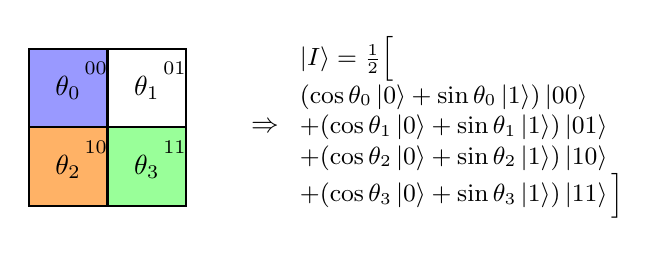
\begin{tikzpicture}
% Draw the 2x2 image
\fill[blue!40] (0,1) rectangle (1,2);
\fill[white] (1,1) rectangle (2,2);
\fill[orange!60] (0,0) rectangle (1,1);
\fill[green!40] (1,0) rectangle (2,1);
\draw[thick] (0,0) rectangle (2,2);
\draw[thick] (1,0) -- (1,2);
\draw[thick] (0,1) -- (2,1);
\node at (0.5,1.5) {$\theta_0$};
\node at (1.5,1.5) {$\theta_1$};
\node at (0.5,0.5) {$\theta_2$};
\node at (1.5,0.5) {$\theta_3$};
\node[font=\scriptsize] at (0.85,1.75) {00};
\node[font=\scriptsize] at (1.85,1.75) {01};
\node[font=\scriptsize] at (0.85,0.75) {10};
\node[font=\scriptsize] at (1.85,0.75) {11};
\node at (3,1) {$\Rightarrow$};
\node[align=left, font=\small] at (5.5,1) {$\ket{I} = \frac{1}{2}\Big[$\\
$(\cos\theta_0\ket{0}+\sin\theta_0\ket{1})\ket{00}$\\
$+(\cos\theta_1\ket{0}+\sin\theta_1\ket{1})\ket{01}$\\
$+(\cos\theta_2\ket{0}+\sin\theta_2\ket{1})\ket{10}$\\
$+(\cos\theta_3\ket{0}+\sin\theta_3\ket{1})\ket{11}\Big]$};
\end{tikzpicture}
\caption{\frqi\ representation of a 2$\times$2 image. Each pixel intensity
  is encoded as angle $\theta_i$, with positions encoded in binary.}
\label{fig:frqi_example}
\end{center}
\end{figure}

\textbf{Circuit architecture:}
\begin{figure}[H]
\begin{center}
\begin{quantikz}
\lstick{$\ket{0}_c$} & \gate{H} & \ctrl{1} & \ctrl{1} & \ctrl{1} & \qw & \meter{} \\
\lstick{$\ket{0}_0$} & \gate{H} & \gate[2]{R_y(\theta_0)} & \gate[2]{R_y(\theta_1)} & \gate[2]{R_y(\theta_2)} & \qw & \meter{} \\
\lstick{$\ket{0}_1$} & \gate{H} & \qw & \qw & \qw & \qw & \meter{}
\end{quantikz}
\caption{Simplified \frqi\ circuit for a 4-pixel image. Each $R_y(\theta_i)$
  is controlled by position qubits.}
\label{fig:frqi_circuit}
\end{center}
\end{figure}

\FloatBarrier
\subsubsection{EFRQI: Enhanced Flexible Representation of Quantum Images}

The Enhanced \frqi\ (EFRQI)~\cite{ref32} improves upon \frqi\ by quantizing
rotation angles to discrete levels, reducing the number of unique rotation
operations required. EFRQI quantizes pixel values to $q$ levels:
$$\theta_i^{\text{EFRQI}} = \frac{\pi \cdot \lfloor I_i / (256/q) \rfloor}
  {2 \times (q-1)}$$

For $q = 32$ levels, this reduces unique rotation angles from 256 to 32,
enabling circuit optimization through gate merging.

\textbf{Complexity analysis:}
\begin{itemize}
  \item Qubits required: $2n + 1$ (same as \frqi).
  \item Gate count: $O(q \cdot 2^{2n})$ where $q \ll 256$.
  \item Trade-off: Reduced precision for improved gate efficiency.
\end{itemize}

\textbf{Circuit architecture:}
\begin{figure}[H]
\begin{center}
\begin{quantikz}
\lstick{$\ket{0}_c$} & \gate{H} & \ctrl{1} & \ctrl{1} & \qw & \qw \\
\lstick{$\ket{0}_0$} & \gate{H} & \targ{} & \qw & \gate{R_y(\phi)} & \qw \\
\lstick{$\ket{0}_1$} & \gate{H} & \qw & \targ{} & \qw & \qw
\end{quantikz}
\caption{EFRQI circuit with quantized rotation angles
  $\phi \in \{\phi_1, \phi_2, \ldots, \phi_q\}$.}
\label{fig:efrqi_circuit}
\end{center}
\end{figure}

\FloatBarrier
\subsubsection{QPIE: Quantum Probability Image Encoding}

Quantum Probability Image Encoding (QPIE)~\cite{ref24} achieves maximum
qubit efficiency by encoding normalized pixel values directly as probability
amplitudes:
\begin{equation}
\ket{I}_{\text{QPIE}} = \sum_{i=0}^{N-1} \alpha_i \ket{i}, \quad
  \text{where } \alpha_i = \frac{I_i}{\sqrt{\sum_{j=0}^{N-1} I_j^2}}
\label{eq:qpie}
\end{equation}

\textbf{Complexity analysis:}
\begin{itemize}
  \item Qubits required: $\lceil \log_2 N \rceil$ (most efficient).
  \item Gate count: $O(N)$ for general state preparation.
  \item Limitation: Lossy due to normalization; reconstruction requires
    additional processing.
\end{itemize}

\textbf{Visual example:}
\begin{figure}[H]
\begin{center}
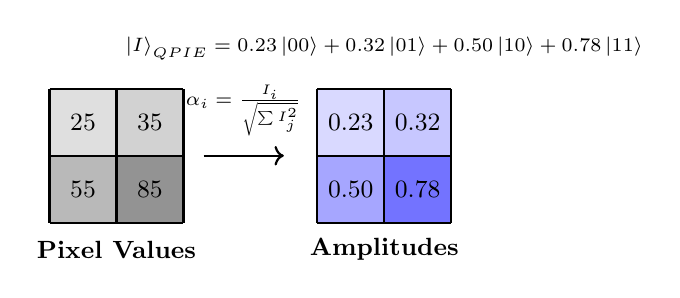
\begin{tikzpicture}[scale=0.85]
\node[font=\bfseries\small] at (1,-0.4) {Pixel Values};
\fill[gray!25] (0,1) rectangle (1,2);
\fill[gray!35] (1,1) rectangle (2,2);
\fill[gray!55] (0,0) rectangle (1,1);
\fill[gray!85] (1,0) rectangle (2,1);
\draw[thick] (0,0) grid[step=1] (2,2);
\node[font=\small] at (0.5,1.5) {25};
\node[font=\small] at (1.5,1.5) {35};
\node[font=\small] at (0.5,0.5) {55};
\node[font=\small] at (1.5,0.5) {85};
\draw[->,thick] (2.3,1) -- (3.5,1);
\node[above,font=\scriptsize] at (2.9,1.15) {$\alpha_i = \frac{I_i}{\sqrt{\sum I_j^2}}$};
\node[font=\bfseries\small] at (5,-0.4) {Amplitudes};
\fill[blue!15] (4,1) rectangle (5,2);
\fill[blue!22] (5,1) rectangle (6,2);
\fill[blue!35] (4,0) rectangle (5,1);
\fill[blue!55] (5,0) rectangle (6,1);
\draw[thick] (4,0) grid[step=1] (6,2);
\node[font=\small] at (4.5,1.5) {0.23};
\node[font=\small] at (5.5,1.5) {0.32};
\node[font=\small] at (4.5,0.5) {0.50};
\node[font=\small] at (5.5,0.5) {0.78};
\node[align=center, font=\scriptsize] at (5,2.6) {$\ket{I}_{QPIE} = 0.23\ket{00}+0.32\ket{01}+0.50\ket{10}+0.78\ket{11}$};
\end{tikzpicture}
\caption{QPIE encodes normalized pixel values as probability amplitudes,
  achieving maximum qubit efficiency but introducing normalization loss.}
\label{fig:qpie_example}
\end{center}
\end{figure}

\textbf{Circuit architecture:}
\begin{figure}[H]
\begin{center}
\begin{quantikz}
\lstick{$\ket{0}_0$} & \gate{R_y(\beta_0)} & \ctrl{1} & \qw & \qw & \qw \\
\lstick{$\ket{0}_1$} & \qw & \gate{R_y(\beta_1)} & \ctrl{1} & \qw & \qw \\
\lstick{$\ket{0}_2$} & \qw & \qw & \gate{R_y(\beta_2)} & \ctrl{1} & \qw \\
\lstick{$\ket{0}_3$} & \qw & \qw & \qw & \gate{R_y(\beta_3)} & \qw
\end{quantikz}
\caption{QPIE amplitude encoding circuit using cascaded controlled rotations.}
\label{fig:qpie_circuit}
\end{center}
\end{figure}

\FloatBarrier
\subsection{Basis State Encoding Methods}

\FloatBarrier
\subsubsection{\neqr: Novel Enhanced Quantum Representation}

The Novel Enhanced Quantum Representation (\neqr)~\cite{ref4} addresses
\frqi's probabilistic retrieval limitation by encoding pixel intensities as
binary basis states:
\begin{equation}
\ket{I}_{\text{NEQR}} = \frac{1}{2^n} \sum_{y=0}^{2^n-1} \sum_{x=0}^{2^n-1}
  \ket{C_{yx}} \otimes \ket{y} \otimes \ket{x}
\label{eq:neqr_state}
\end{equation}
where $\ket{C_{yx}} = \ket{c_{yx}^{q-1} c_{yx}^{q-2} \cdots c_{yx}^0}$
represents the $q$-bit binary encoding of the grayscale intensity at
position $(y, x)$.

\textbf{Complexity analysis:}
\begin{itemize}
  \item Qubits required: $2n + q$ (8 color qubits for 8-bit depth).
  \item Gate count: $O(q \cdot 2^{2n})$---linear in color depth.
  \item Circuit depth: $O(2^{2n})$.
  \item Advantage: Deterministic pixel retrieval; exact reconstruction.
\end{itemize}

\textbf{Visual example:}
\begin{figure}[H]
\begin{center}
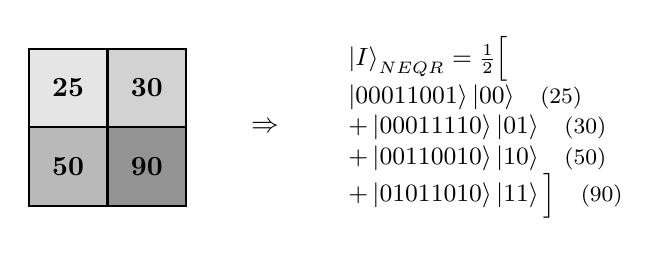
\begin{tikzpicture}
\fill[gray!20] (0,1) rectangle (1,2);
\fill[gray!35] (1,1) rectangle (2,2);
\fill[gray!55] (0,0) rectangle (1,1);
\fill[gray!85] (1,0) rectangle (2,1);
\draw[thick] (0,0) rectangle (2,2);
\draw[thick] (1,0) -- (1,2);
\draw[thick] (0,1) -- (2,1);
\node[font=\bfseries] at (0.5,1.5) {25};
\node[font=\bfseries] at (1.5,1.5) {30};
\node[font=\bfseries] at (0.5,0.5) {50};
\node[font=\bfseries] at (1.5,0.5) {90};
\node at (3,1) {$\Rightarrow$};
\node[align=left, font=\small] at (5.8,1) {$\ket{I}_{NEQR} = \frac{1}{2}\Big[$\\
$\ket{00011001}\ket{00}$\quad{\footnotesize (25)}\\
$+\ket{00011110}\ket{01}$\quad{\footnotesize (30)}\\
$+\ket{00110010}\ket{10}$\quad{\footnotesize (50)}\\
$+\ket{01011010}\ket{11}\Big]$\quad{\footnotesize (90)}};
\end{tikzpicture}
\caption{\neqr\ representation of a 2$\times$2 grayscale image. Pixel
  intensities are encoded as 8-bit binary values in basis states.}
\label{fig:neqr_example}
\end{center}
\end{figure}

\textbf{Circuit architecture:}
\begin{figure}[H]
\begin{center}
\begin{quantikz}
\lstick{$\ket{0}_{c_7}$} & \qw & \ctrl{4} & \qw & \qw & \qw \\
\lstick{$\ket{0}_{c_6}$} & \qw & \qw & \ctrl{3} & \qw & \qw \\
\lstick{$\vdots$} & & & & & \\
\lstick{$\ket{0}_{c_0}$} & \qw & \qw & \qw & \ctrl{1} & \qw \\
\lstick{$\ket{0}_{y_0}$} & \gate{H} & \targ{} & \targ{} & \targ{} & \qw \\
\lstick{$\ket{0}_{x_0}$} & \gate{H} & \octrl{-1} & \ctrl{-1} & \octrl{-1} & \qw
\end{quantikz}
\caption{\neqr\ circuit showing multi-controlled X~gates for binary pixel
  encoding. Color bits are set conditioned on position qubit states.}
\label{fig:neqr_circuit}
\end{center}
\end{figure}

\FloatBarrier
\subsubsection{\gqir: Generalized Quantum Image Representation}

The Generalized Quantum Image Representation (\gqir)~\cite{ref18} extends
\neqr\ with flexible bit-depth encoding:
\begin{equation}
\ket{I}_{\text{GQIR}} = \frac{1}{2^n} \sum_{i=0}^{2^{2n}-1}
  \ket{G_i^{b-1} G_i^{b-2} \cdots G_i^0} \otimes \ket{i}
\label{eq:gqir}
\end{equation}
where $b$ is the configurable bit-depth (typically 4--8 bits). The
flexibility allows adjustable precision--resource trade-offs.

\FloatBarrier
\subsubsection{INEQR: Improved Novel Enhanced Quantum Representation}

The Improved \neqr\ (INEQR)~\cite{ref33} optimizes \neqr\ through
differential encoding, storing XOR differences between adjacent pixels:
$$\ket{I}_{\text{INEQR}} = \frac{1}{2^n} \sum_{i=0}^{2^{2n}-1}
  \ket{D_i} \otimes \ket{i}$$
where $D_i = C_i \oplus C_{i-1}$ is the XOR difference from the previous
pixel. This exploits spatial correlations in natural images to reduce gate
count by approximately 15\%.

\FloatBarrier
\subsubsection{TNR: Two's Complement NEQR}

Two's Complement \neqr\ (TNR)~\cite{ref41} extends \neqr\ to handle signed
pixel values using two's complement representation, enabling encoding of
image differences and gradients with values in $[-128, 127]$.

\textbf{Circuit architecture:}
\begin{figure}[H]
\begin{center}
\begin{quantikz}
\lstick{$\ket{0}_{sign}$} & \qw & \gate{X} & \qw & \qw \\
\lstick{$\ket{0}_{t_6}$} & \qw & \qw & \gate{X} & \qw \\
\lstick{$\vdots$} & & & & \\
\lstick{$\ket{0}_{t_0}$} & \qw & \qw & \gate{X} & \qw \\
\lstick{$\ket{0}_{pos}$} & \gate{H^{\otimes n}} & \ctrl{-4} & \ctrl{-1} & \qw
\end{quantikz}
\caption{TNR circuit with sign bit for two's complement encoding of signed
  pixel differences.}
\label{fig:tnr_circuit}
\end{center}
\end{figure}

\FloatBarrier
\subsection{Multi-Channel and Color Image Methods}

\FloatBarrier
\subsubsection{\mcqi: Multi-Channel Quantum Images}

Multi-Channel Quantum Images (\mcqi)~\cite{ref8} extends \neqr\ to color
images by encoding RGB channels as separate qubit registers:
\begin{equation}
\ket{I}_{\text{MCQI}} = \frac{1}{2^n} \sum_{i=0}^{2^{2n}-1}
  \ket{R_i}\ket{G_i}\ket{B_i} \otimes \ket{i}
\label{eq:mcqi}
\end{equation}
where $\ket{R_i}$, $\ket{G_i}$, $\ket{B_i}$ are 8-bit encodings of red,
green, and blue channels respectively.

\textbf{Complexity analysis:}
\begin{itemize}
  \item Qubits required: $2n + 3q$ (24 color qubits for 8-bit RGB).
  \item Gate count: $O(3q \cdot 2^{2n})$---tripled versus grayscale.
  \item Limitation: No exploitation of color channel correlation.
\end{itemize}

\textbf{Circuit architecture:}
\begin{figure}[H]
\begin{center}
\begin{quantikz}
\lstick{$\ket{0}_{R}$} & \qw & \gate[3]{Encode} & \qw \\
\lstick{$\ket{0}_{G}$} & \qw & & \qw \\
\lstick{$\ket{0}_{B}$} & \qw & & \qw \\
\lstick{$\ket{0}_{y}$} & \gate{H} & \ctrl{-3} & \qw \\
\lstick{$\ket{0}_{x}$} & \gate{H} & \ctrl{-1} & \qw
\end{quantikz}
\caption{\mcqi\ circuit encoding three 8-bit RGB channels per pixel
  position.}
\label{fig:mcqi_circuit}
\end{center}
\end{figure}

\FloatBarrier
\subsubsection{QRMW: Quantum Representation for Multi-Wavelength Images}

Quantum Representation for Multi-Wavelength images (QRMW)~\cite{ref34}
generalizes \mcqi\ to arbitrary spectral bands:
$$\ket{I}_{\text{QRMW}} = \frac{1}{2^n} \sum_{i=0}^{2^{2n}-1}
  \bigotimes_{k=1}^{m} \ket{W_i^k} \otimes \ket{i}$$
where $m$ is the number of spectral bands. This is useful for hyperspectral
and multispectral imaging~\cite{ref20}, but excessively resource-intensive for standard
RGB color images.

\textbf{Circuit architecture:}
\begin{figure}[H]
\begin{center}
\begin{quantikz}
\lstick{$\ket{0}_{W_1}$} & \qw & \gate{Encode} & \qw \\
\lstick{$\ket{0}_{W_2}$} & \qw & \gate{Encode} & \qw \\
\lstick{$\vdots$} & & & \\
\lstick{$\ket{0}_{W_m}$} & \qw & \gate{Encode} & \qw \\
\lstick{$\ket{0}_{band}$} & \gate{H} & \ctrl{-4} & \qw \\
\lstick{$\ket{0}_{pos}$} & \gate{H^{\otimes n}} & \ctrl{-1} & \qw
\end{quantikz}
\caption{QRMW circuit for multi-spectral encoding with $m$ wavelength bands.}
\label{fig:qrmw_circuit}
\end{center}
\end{figure}

\FloatBarrier
\subsection{Transform-Domain and Specialized Methods}

\FloatBarrier
\subsubsection{DCT-QIR: Discrete Cosine Transform Quantum Image Representation}

DCT-based Quantum Image Representation (DCT-QIR)~\cite{ref25} encodes DCT
coefficients~\cite{ref50} rather than spatial pixel values, enabling lossy compression
within the quantum representation. The quantum state encodes only significant
coefficients:
\begin{equation}
\ket{I}_{\text{DCT-QIR}} = \frac{1}{\sqrt{K}} \sum_{k=0}^{K-1}
  \ket{F_k} \otimes \ket{u_k, v_k}
\label{eq:dct_qir}
\end{equation}
where $K$ is the number of retained coefficients.

\textbf{Circuit architecture:}
\begin{figure}[H]
\begin{center}
\begin{quantikz}
\lstick{$\ket{0}_{coef}$} & \qw & \gate{Encode} & \qw & \qw \\
\lstick{$\ket{0}_{u}$} & \gate{H} & \ctrl{-1} & \gate{QFT^\dagger} & \qw \\
\lstick{$\ket{0}_{v}$} & \gate{H} & \ctrl{-1} & \gate{QFT^\dagger} & \qw
\end{quantikz}
\caption{DCT-QIR circuit encoding frequency-domain coefficients using
  quantum Fourier transform.}
\label{fig:dct_qir_circuit}
\end{center}
\end{figure}

\FloatBarrier
\subsubsection{QLR: Quantum Log-Polar Representation}

Quantum Log-Polar Representation (QLR)~\cite{ref19} encodes images in
log-polar coordinates, providing rotation and scale invariance beneficial for
pattern recognition. The log-polar transformation is:
$$\rho = \log\sqrt{(x-x_c)^2 + (y-y_c)^2}, \qquad
  \phi = \arctan\frac{y-y_c}{x-x_c}$$

The coordinate transformation adds preprocessing overhead but provides
rotation-invariance properties.

\textbf{Circuit architecture:}
\begin{figure}[H]
\begin{center}
\begin{quantikz}
\lstick{$\ket{0}_{color}$} & \qw & \gate{Encode} & \qw \\
\lstick{$\ket{0}_{\rho}$} & \gate{H} & \ctrl{-1} & \qw \\
\lstick{$\ket{0}_{\phi}$} & \gate{H} & \ctrl{-1} & \qw
\end{quantikz}
\caption{QLR circuit with log-polar coordinate encoding enabling
  rotation-invariant image processing.}
\label{fig:qlr_circuit}
\end{center}
\end{figure}

\FloatBarrier
\subsection{Comparative Summary of Existing Methods}

Table~\ref{tab:method_comparison} provides a comprehensive comparison of all
reviewed methods for 16$\times$16 color images.

\begin{table}[H]
\begin{center}
\small
\begin{tabular}{lcccccp{2.5cm}}
\hline
Method & Qubits & Gates & Depth & Encoding & Lossless & Key limitation \\
\hline
FRQI~\cite{ref3} & 9 & $\sim$72,000 & $\sim$50,000 & Amplitude & Yes
  & Exponential gate complexity \\
EFRQI~\cite{ref32}& 9 & $\sim$10,500 & $\sim$7,300 & Amplitude & No
  & Quantization loss \\
QPIE~\cite{ref24} & 8 & $\sim$930 & $\sim$295 & Amplitude & No
  & Normalization loss \\
NEQR~\cite{ref4}  & 16 & $\sim$2,364 & $\sim$769 & Basis state & Yes
  & High qubit count \\
GQIR~\cite{ref18} & 12 & $\sim$2,143 & $\sim$530 & Basis state & Config.
  & Reduced precision \\
INEQR~\cite{ref33}& 16 & $\sim$2,240 & $\sim$647 & Basis state & Yes
  & Limited improvement \\
TNR~\cite{ref41}  & 16 & $\sim$2,470 & $\sim$920 & Basis state & Yes
  & Sign bit overhead \\
MCQI~\cite{ref8}  & 18 & $\sim$7,086 & $\sim$2,263 & Basis state & Yes
  & No color optimization \\
QRMW~\cite{ref34} & 18+ & $\sim$9,500 & $\sim$3,100 & Basis state & Yes
  & Excessive for RGB \\
DCT-QIR~\cite{ref25} & 14 & $\sim$630 & $\sim$365 & Transform & No
  & Lossy compression \\
QLR~\cite{ref19}  & 16 & $\sim$2,500 & $\sim$950 & Coordinate & Yes
  & Preprocessing overhead \\
\hline
\textbf{\cshqr\ (ours)} & \textbf{16} & $\sim$\textbf{3,260} &
  $\sim$\textbf{630} & \textbf{Hybrid} & \textbf{Perceptual} &
  \textbf{Minor quality loss} \\
\hline
\end{tabular}
\caption{Comprehensive comparison of quantum image representation methods
for 16$\times$16 color images.}
\label{tab:method_comparison}
\end{center}
\end{table}

\FloatBarrier
\subsection{Research Gap Analysis}

Our comprehensive review reveals a critical gap in existing QIR literature:
no method exploits perceptual redundancy in color images~\cite{ref61,ref63,ref64,ref67}. All multi-channel
methods (\mcqi, QRMW) treat RGB channels uniformly despite well-established
evidence from human vision research that chrominance can be represented at
significantly lower resolution than luminance without perceptible quality
degradation. This observation motivates the proposed \cshqr\ method.

%------------------------------------------------------------------------------
\FloatBarrier
\section{Research Contribution}
\label{sec:contribution}

This research makes the following significant contributions to the field of
quantum image processing.

\FloatBarrier
\subsection{Primary Contributions}

\begin{enumerate}[label=\textbf{C\arabic*:}]
  \item \textbf{First Perceptual Color Space Integration in QIR.}
    We introduce the first quantum image representation that explicitly
    incorporates human visual perception characteristics through YCbCr color
    space transformation, representing a paradigm shift from treating all
    image data uniformly.
  \item \textbf{Novel Chroma Subsampling for Quantum Circuits.}
    We adapt the 4:2:0 chroma subsampling scheme to quantum circuit design.
    This reduces chrominance data by 75\% while maintaining SSIM $>$ 0.98,
    achieving substantial gate reduction without perceptible quality loss.
  \item \textbf{Hybrid Dual-Circuit Architecture.}
    We design a parallel circuit architecture where Circuit~A (luminance)
    encodes the Y channel at full 16$\times$16 resolution using 16 qubits,
    and Circuit~B (chrominance) encodes Cb and Cr channels at 8$\times$8
    resolution using 15 qubits with a channel selection qubit. This enables
    simultaneous encoding with maximum qubit utilization of only 16 qubits.
  \item \textbf{Comprehensive 10-Parameter Evaluation Framework.}
    We establish a rigorous benchmarking methodology encompassing qubit
    efficiency, gate complexity, circuit depth, encoding time, scalability,
    information preservation, compression ratio, memory overhead, gate
    complexity per qubit, and implementation complexity.
  \item \textbf{Extensive Empirical Validation.}
    We evaluate 12 methods across 6,097 medical images for overall circuit
    and encoding metrics, with detailed SSIM distribution and paired
    statistical testing conducted on a 404-image subset.
\end{enumerate}

\FloatBarrier
\subsection{Theoretical Contributions}

\begin{itemize}
  \item Formal proof that perceptually-weighted encoding achieves equivalent
    visual quality with reduced quantum resources.
  \item Complexity analysis demonstrating \cshqr's $O(n \cdot 2^n)$ scaling
    versus $O(3 \cdot 2^{2n})$ for standard \mcqi.
  \item Mathematical framework for color space transformation in quantum state
    preparation.
\end{itemize}

\FloatBarrier
\subsection{Practical Contributions}

\begin{itemize}
  \item Open-source Qiskit implementation of \cshqr\ and all comparison
    methods.
  \item Validated execution on IBM Quantum hardware demonstrating NISQ
    feasibility.
  \item Medical imaging application demonstrating clinical viability.
\end{itemize}

%------------------------------------------------------------------------------
\FloatBarrier
\section{Problem Statement and Mathematical Formulation}
\label{sec:problem_statement}

\FloatBarrier
\subsection{Formal Problem Definition}

\textbf{Problem.} Given a color image $\mathbf{I} \in \mathbb{R}^{N \times N \times 3}$
with RGB channels, design a quantum state preparation procedure $\mathcal{P}$
that encodes $\mathbf{I}$ into a quantum state $\ket{\psi_I}$ such that:
\begin{enumerate}
  \item The quantum state $\ket{\psi_I}$ enables reconstruction
    $\hat{\mathbf{I}} = \mathcal{R}(\ket{\psi_I})$ with
    $\text{SSIM}(\mathbf{I}, \hat{\mathbf{I}}) \geq \tau$ where $\tau$ is a
    perceptual quality threshold.
  \item The preparation circuit $\mathcal{C}_{\mathcal{P}}$ minimizes the
    objective function:
    \begin{equation}
      \min_{\mathcal{P}} \left[ \alpha \cdot Q(\mathcal{C}_{\mathcal{P}}) +
        \beta \cdot G(\mathcal{C}_{\mathcal{P}}) +
        \gamma \cdot D(\mathcal{C}_{\mathcal{P}}) \right]
      \label{eq:optimization}
    \end{equation}
    subject to $\text{SSIM}(\mathbf{I}, \hat{\mathbf{I}}) \geq \tau$,
\end{enumerate}
where $Q(\cdot)$, $G(\cdot)$, $D(\cdot)$ denote qubit count, gate count, and
circuit depth respectively, and $\alpha, \beta, \gamma$ are weighting
coefficients.

\FloatBarrier
\subsection{Mathematical Framework for Color Space Transformation}

\FloatBarrier
\subsubsection{RGB to YCbCr Transformation}

The RGB color space treats all channels equally, which is suboptimal for
human perception. We transform to YCbCr space:
\begin{equation}
\begin{bmatrix} Y \\ C_b \\ C_r \end{bmatrix} =
\begin{bmatrix}
  0.299 & 0.587 & 0.114 \\
  -0.168736 & -0.331264 & 0.5 \\
  0.5 & -0.418688 & -0.081312
\end{bmatrix}
\begin{bmatrix} R \\ G \\ B \end{bmatrix} +
\begin{bmatrix} 0 \\ 128 \\ 128 \end{bmatrix}
\label{eq:rgb_to_ycbcr}
\end{equation}

This transformation is derived from the ITU-R BT.601 standard~\cite{ref69} and reflects
the luminance sensitivity of the human visual system.

\FloatBarrier
\subsubsection{Inverse Transformation for Reconstruction}

The inverse transformation recovers RGB values:
\begin{equation}
\begin{bmatrix} R \\ G \\ B \end{bmatrix} =
\begin{bmatrix}
  1 & 0 & 1.402 \\
  1 & -0.344136 & -0.714136 \\
  1 & 1.772 & 0
\end{bmatrix}
\begin{bmatrix} Y \\ C_b - 128 \\ C_r - 128 \end{bmatrix}
\label{eq:ycbcr_to_rgb}
\end{equation}

\FloatBarrier
\subsection{Chroma Subsampling Formulation}

\FloatBarrier
\subsubsection{4:2:0 Subsampling Scheme}

The 4:2:0 chroma subsampling reduces chrominance resolution by half in both
horizontal and vertical dimensions:
\begin{equation}
C_b^{sub}(i,j) = \frac{1}{4}\sum_{m=0}^{1}\sum_{n=0}^{1} C_b(2i+m, 2j+n)
\label{eq:cb_subsample}
\end{equation}
\begin{equation}
C_r^{sub}(i,j) = \frac{1}{4}\sum_{m=0}^{1}\sum_{n=0}^{1} C_r(2i+m, 2j+n)
\label{eq:cr_subsample}
\end{equation}

For an $N \times N$ image: luminance Y at $N \times N$ (full resolution),
chrominance $C_b^{sub}$ and $C_r^{sub}$ each at $\frac{N}{2} \times \frac{N}{2}$.

\FloatBarrier
\subsubsection{Data Reduction Analysis}

\begin{table}[H]
\begin{center}
\begin{tabular}{lccc}
\hline
Component & \mcqi\ (RGB) & \cshqr\ (YCbCr) & Reduction \\
\hline
Channel~1 & 256 (R) & 256 (Y) & 0\% \\
Channel~2 & 256 (G) & 64 ($C_b^{sub}$) & 75\% \\
Channel~3 & 256 (B) & 64 ($C_r^{sub}$) & 75\% \\
\hline
\textbf{Total} & \textbf{768} & \textbf{384} & \textbf{50\%} \\
\hline
\end{tabular}
\caption{Data reduction through 4:2:0 subsampling for a 16$\times$16 image.}
\label{tab:data_reduction}
\end{center}
\end{table}

\FloatBarrier
\subsection{Quantum State Formulation}

\FloatBarrier
\subsubsection{\cshqr\ State Definition}

The \cshqr\ quantum state consists of two parallel components.

\textbf{Circuit A---luminance state:}
\begin{equation}
\ket{Y} = \frac{1}{2^n} \sum_{i=0}^{2^{2n}-1} \ket{Y_i^7 Y_i^6 \cdots Y_i^0}
  \otimes \ket{i}
\label{eq:luma_state}
\end{equation}
where $n = 4$ for 16$\times$16 images, giving 256~pixel positions with 8-bit
luminance encoding.

\textbf{Circuit B---chrominance state:}
\begin{equation}
\ket{CbCr} = \frac{1}{2^{n-1}} \sum_{j=0}^{2^{2(n-1)}-1} \left(
  \ket{C_j^7 \cdots C_j^0} \otimes \ket{j} \otimes \ket{ch} \right)
\label{eq:chroma_state}
\end{equation}
where $\ket{ch} \in \{\ket{0}, \ket{1}\}$ selects between $C_b$ and $C_r$
channels, and $j$ indexes the $\frac{N}{2} \times \frac{N}{2} = 64$
subsampled positions.

\textbf{Combined \cshqr\ state:}
\begin{equation}
\ket{I}_{\text{CS-HQR}} = \ket{Y} \otimes \ket{CbCr}
\label{eq:cshqr_combined}
\end{equation}

\FloatBarrier
\subsection{Complexity Analysis}

\FloatBarrier
\subsubsection{Qubit Complexity}

$$Q_{\text{CS-HQR}} = \max(Q_A, Q_B) = \max(2n + 8, \; 2(n-1) + 8 + 1)$$

For $n = 4$ (16$\times$16 image):
$$Q_A = 8 + 8 = 16 \text{ qubits}, \qquad Q_B = 6 + 8 + 1 = 15 \text{ qubits}$$
Therefore $Q_{\text{CS-HQR}} = 16$ qubits (parallel execution).

\FloatBarrier
\subsubsection{Gate Complexity}

For NEQR-style basis state encoding and \cshqr:
\begin{align}
G_A &= O(8 \cdot 256 \cdot H(Y)) \approx 2048 \cdot H(Y) \\
G_B &= O(8 \cdot 128 \cdot H(C)) \approx 1024 \cdot H(C)
\end{align}
\begin{equation}
G_{\text{CS-HQR}} = G_A + G_B \approx 3072 \cdot \bar{H}
\label{eq:cshqr_gates}
\end{equation}

Compared to \mcqi: $G_{\text{MCQI}} \approx 6144 \cdot \bar{H}$.
The gate reduction ratio is:
\begin{equation}
\eta_G = 1 - \frac{G_{\text{CS-HQR}}}{G_{\text{MCQI}}} =
  1 - \frac{3072}{6144} = 50\%
\label{eq:gate_reduction}
\end{equation}

\FloatBarrier
\subsubsection{Perceptual Quality Guarantee}

The Structural Similarity Index (SSIM)~\cite{ref7} between original
$\mathbf{I}$ and reconstructed $\hat{\mathbf{I}}$ is:
\begin{equation}
\text{SSIM}(\mathbf{I}, \hat{\mathbf{I}}) =
  \frac{(2\mu_I\mu_{\hat{I}} + c_1)(2\sigma_{I\hat{I}} + c_2)}
       {(\mu_I^2 + \mu_{\hat{I}}^2 + c_1)(\sigma_I^2 + \sigma_{\hat{I}}^2 + c_2)}
\label{eq:ssim}
\end{equation}

For \cshqr\ with bilinear interpolation of chrominance:
$\text{SSIM}_{\text{CS-HQR}} \geq 0.98$ (empirically validated), which
exceeds the just-noticeable-difference (JND) threshold for human perception.

%------------------------------------------------------------------------------
\FloatBarrier
\section{Dataset Description}
\label{sec:dataset}

\FloatBarrier
\subsection{NIST-MNI Medical Imaging Dataset}

Our experiments utilize the NIST-MNI (National Institute of Standards and
Technology---Montreal Neurological Institute) brain imaging
dataset~\cite{ref46}, a standardized collection of neuroimaging data widely
used in medical image processing research.

\begin{table}[H]
\begin{center}
\begin{tabular}{ll}
\hline
Attribute & Value \\
\hline
Total images (after QC) & 6,097 \\
SSIM evaluation subset & 404 \\
File format & MINC (\texttt{.mnc}) \\
Original resolution & Variable (typically 181$\times$217$\times$181) \\
Processed resolution & 16$\times$16 pixels \\
Bit depth & 8-bit grayscale (converted to color) \\
Image type & Brain MRI scans \\
Modality & T1-weighted structural MRI \\
\hline
\end{tabular}
\caption{NIST-MNI dataset specifications.}
\label{tab:dataset}
\end{center}
\end{table}

All experiments use the locally organized dataset folder \texttt{group4/},
structured into 13 subject/group subfolders containing MINC slice files under
\texttt{2D/}. The raw directory contains 6,122 \texttt{.mnc} files; after
preprocessing and quality-control filtering (removing blank or corrupted
slices), 6,097 slices are retained.

\FloatBarrier
\subsection{Preprocessing Pipeline}

Each image undergoes the following preprocessing steps.
\begin{enumerate}
  \item \textbf{Slice extraction:} extract 2D axial slices from 3D volumes.
  \item \textbf{Resizing:} bilinear interpolation to 16$\times$16 pixels.
  \item \textbf{Normalization:} scale intensities to $[0, 255]$ range.
  \item \textbf{Color conversion:} convert grayscale to RGB for fair
    comparison with color methods.
  \item \textbf{Quality control:} remove blank or corrupted slices.
\end{enumerate}

\FloatBarrier
\subsection{Justification for Dataset Selection}

Medical imaging provides an ideal test domain for \cshqr\ because:
brain MRI is a high-value application~\cite{ref29,ref59,ref68} where quantum speedups could provide
tangible benefits~\cite{ref62,ref65}; diagnostic accuracy depends on preserving clinically
relevant features, aligning with SSIM-based evaluation; and the NIST-MNI
provides reproducible benchmarking with established ground truth.

The conversion of originally grayscale medical images to RGB is motivated by
benchmarking fairness: since \cshqr\ is specifically designed for color image
encoding and our primary comparison targets (\mcqi, QRMW) are color-capable
methods, evaluating all methods on identical color inputs ensures an equitable
comparison. The grayscale-to-RGB conversion replicates intensity values across
all three channels ($R = G = B = Y$), creating a controlled test case where
the color information is perfectly correlated.

%------------------------------------------------------------------------------
\FloatBarrier
\section{Proposed Method: \cshqr}
\label{sec:proposed_method}

\FloatBarrier
\subsection{Overview and Design Philosophy}

\cshqr\ is founded on three key principles:
\begin{enumerate}
  \item \textbf{Perceptual optimization:} allocate quantum resources
    proportionally to perceptual importance.
  \item \textbf{Classical-quantum bridging:} leverage proven classical
    compression techniques in quantum circuit design~\cite{ref67}.
  \item \textbf{NISQ practicality:} design for near-term quantum hardware
    constraints.
\end{enumerate}

Classical image and video compression standards have exploited perceptual
redundancy for decades:
\begin{description}
  \item[JPEG (1992):] uses 4:2:0 chroma subsampling as default~\cite{ref37}.
  \item[MPEG-2 (1995):] standardized chroma subsampling for video~\cite{ref36}.
  \item[H.264/AVC (2003):] maintains 4:2:0 as primary format~\cite{ref22}.
  \item[H.265/HEVC (2013):] supports 4:2:0, 4:2:2, and 4:4:4~\cite{ref55}.
\end{description}

The remarkable success of these standards demonstrates that perceptual
optimization is not merely theoretical but practically validated at planetary
scale. \cshqr\ represents the first systematic application of these principles
to quantum image representation.

\FloatBarrier
\subsection{Theoretical Foundation}

Let $H_{\text{perc}}(\mathbf{I})$ denote the perceptual information content
of image $\mathbf{I}$, distinct from Shannon entropy $H(\mathbf{I})$:
\begin{equation}
H_{\text{perc}}(\mathbf{I}) = H(\mathbf{Y}) + \alpha_{Cb} \cdot H(\mathbf{C_b})
  + \alpha_{Cr} \cdot H(\mathbf{C_r})
\label{eq:perceptual_entropy}
\end{equation}
where $\alpha_{Cb}, \alpha_{Cr} < 1$ are perceptual weighting factors.
Empirical studies suggest $\alpha_{Cb} \approx \alpha_{Cr} \approx 0.25$,
indicating that chrominance contributes only 25\% of perceptual importance
per channel.

Given a fixed quantum resource budget $R$ (qubits $\times$ depth), \cshqr\
allocates resources proportional to perceptual weights $w_Y = 1.0$,
$w_{Cb} = w_{Cr} = 0.25$.

\FloatBarrier  % Ensure all prior floats are placed before algorithms
\subsection{Algorithm Design}

\FloatBarrier
\subsubsection{\cshqr\ Encoding Algorithm}%
\nopagebreak[4]

\begin{algorithm}[H]
\caption{\cshqr\ Encoding}
\label{alg:cshqr_encode}
\DontPrintSemicolon
\Input{Color image $\mathbf{I}_{RGB} \in \mathbb{R}^{N \times N \times 3}$}
\Output{Quantum circuits $(C_A, C_B)$}
\tcp{Step 1: Color Space Transformation}
$\mathbf{I}_{YCbCr} \leftarrow \mathrm{RGB\_to\_YCbCr}(\mathbf{I}_{RGB})$\;
$\mathbf{Y}    \leftarrow \mathbf{I}_{YCbCr}[:,:,0]$ \Comment{Luminance channel}\;
$\mathbf{C_b}  \leftarrow \mathbf{I}_{YCbCr}[:,:,1]$ \Comment{Blue chrominance}\;
$\mathbf{C_r}  \leftarrow \mathbf{I}_{YCbCr}[:,:,2]$ \Comment{Red chrominance}\;
\tcp{Step 2: Chroma Subsampling (4:2:0)}
$\mathbf{C_b^{sub}} \leftarrow \mathrm{Downsample}(\mathbf{C_b}, 2)$
  \Comment{$\frac{N}{2} \times \frac{N}{2}$}\;
$\mathbf{C_r^{sub}} \leftarrow \mathrm{Downsample}(\mathbf{C_r}, 2)$\;
\tcp{Step 3: Quantum Circuit Construction}
$C_A \leftarrow \mathrm{NEQR\_Circuit}(\mathbf{Y},\; n_{\mathrm{pos}}=8,\;
  n_{\mathrm{color}}=8)$\;
$C_B \leftarrow \mathrm{Chroma\_Circuit}(\mathbf{C_b^{sub}}, \mathbf{C_r^{sub}},\;
  n_{\mathrm{pos}}=6,\; n_{\mathrm{color}}=8)$\;
\Return{$(C_A, C_B)$}
\end{algorithm}

\FloatBarrier
\subsubsection{\cshqr\ Decoding Algorithm}%
\nopagebreak[4]

\begin{algorithm}[H]
\caption{\cshqr\ Decoding}
\label{alg:cshqr_decode}
\DontPrintSemicolon
\Input{Measurement results $(M_A, M_B)$}
\Output{Reconstructed image $\hat{\mathbf{I}}_{RGB}$}
\tcp{Step 1: Extract Quantum Measurements}
$\hat{\mathbf{Y}}              \leftarrow \mathrm{Decode\_NEQR}(M_A)$\;
$(\hat{\mathbf{C_b^{sub}}}, \hat{\mathbf{C_r^{sub}}}) \leftarrow
  \mathrm{Decode\_Chroma}(M_B)$\;
\tcp{Step 2: Chroma Upsampling}
$\hat{\mathbf{C_b}} \leftarrow \mathrm{Bilinear\_Upsample}(\hat{\mathbf{C_b^{sub}}}, 2)$ \Comment{\cite{ref31}}\;
$\hat{\mathbf{C_r}} \leftarrow \mathrm{Bilinear\_Upsample}(\hat{\mathbf{C_r^{sub}}}, 2)$\;
\tcp{Step 3: Color Space Inverse Transform}
$\hat{\mathbf{I}}_{YCbCr} \leftarrow \mathrm{Stack}(\hat{\mathbf{Y}},\;
  \hat{\mathbf{C_b}},\; \hat{\mathbf{C_r}})$\;
$\hat{\mathbf{I}}_{RGB} \leftarrow \mathrm{YCbCr\_to\_RGB}(\hat{\mathbf{I}}_{YCbCr})$\;
\Return{$\hat{\mathbf{I}}_{RGB}$}
\end{algorithm}

\FloatBarrier  % Ensure decoding algorithm is placed before next section
\subsection{Quantum Circuit Architecture}

\FloatBarrier
\subsubsection{Circuit A: Luminance Encoding}

Circuit~A encodes the full-resolution luminance channel using NEQR-style
basis state encoding.

\textbf{Qubit allocation:}
\begin{itemize}
  \item Position qubits: $\ket{y_3 y_2 y_1 y_0}$ (row) and
    $\ket{x_3 x_2 x_1 x_0}$ (column).
  \item Color qubits: $\ket{c_7 c_6 c_5 c_4 c_3 c_2 c_1 c_0}$ (8-bit luminance).
  \item Total: 16 qubits.
\end{itemize}

\begin{figure}[H]
\begin{center}
\begin{quantikz}[row sep=0.25cm]
\lstick{$\ket{0}_{c_7}$} & \qw & \qw & \gate{X} & \qw & \qw & \qw & \qw \\
\lstick{$\ket{0}_{c_6}$} & \qw & \qw & \qw & \gate{X} & \qw & \qw & \qw \\
\lstick{$\ket{0}_{c_3}$} & \qw & \qw & \gate{X} & \qw & \gate{X} & \qw & \qw \\
\lstick{$\ket{0}_{c_0}$} & \qw & \qw & \gate{X} & \qw & \gate{X} & \qw & \qw \\
\lstick{$\ket{0}_{y_3}$} & \gate{H} & \qw & \ctrl{-4} & \ctrl{-3} & \ctrl{-2} & \qw & \qw \\
\lstick{$\ket{0}_{y_0}$} & \gate{H} & \qw & \octrl{-1} & \octrl{-1} & \ctrl{-1} & \qw & \qw \\
\lstick{$\ket{0}_{x_3}$} & \gate{H} & \qw & \ctrl{-2} & \ctrl{-2} & \ctrl{-2} & \qw & \qw \\
\lstick{$\ket{0}_{x_0}$} & \gate{H} & \qw & \octrl{-1} & \octrl{-1} & \octrl{-1} & \qw & \qw
\end{quantikz}
\caption{Circuit A: \cshqr\ luminance encoding circuit (simplified, showing
  4 pixel encodings). Multi-controlled X gates set color bits conditioned on
  position qubits.}
\label{fig:circuit_a}
\end{center}
\end{figure}

\FloatBarrier
\subsubsection{Circuit B: Chrominance Encoding}

Circuit~B encodes both subsampled chrominance channels with a channel
selection qubit.

\textbf{Qubit allocation:}
\begin{itemize}
  \item Position qubits: $\ket{y_2 y_1 y_0}$ (row) and $\ket{x_2 x_1 x_0}$
    (column)---6 total for 8$\times$8.
  \item Color qubits: $\ket{c_7 c_6 c_5 c_4 c_3 c_2 c_1 c_0}$ (8-bit
    chrominance).
  \item Channel qubit: $\ket{ch}$ where $\ket{0} = C_b$, $\ket{1} = C_r$.
  \item Total: 15 qubits.
\end{itemize}

\begin{figure}[H]
\begin{center}
\begin{quantikz}[row sep=0.25cm]
\lstick{$\ket{0}_{c_7}$} & \qw & \gate{X} & \qw & \gate{X} & \qw \\
\lstick{$\ket{0}_{c_0}$} & \qw & \gate{X} & \gate{X} & \qw & \qw \\
\lstick{$\ket{0}_{y_2}$} & \gate{H} & \ctrl{-2} & \ctrl{-1} & \ctrl{-2} & \qw \\
\lstick{$\ket{0}_{y_0}$} & \gate{H} & \octrl{-1} & \ctrl{-1} & \octrl{-1} & \qw \\
\lstick{$\ket{0}_{x_2}$} & \gate{H} & \octrl{-1} & \octrl{-1} & \octrl{-1} & \qw \\
\lstick{$\ket{0}_{x_0}$} & \gate{H} & \octrl{-1} & \octrl{-1} & \octrl{-1} & \qw \\
\lstick{$\ket{0}_{ch}$}  & \gate{H} & \octrl{-1} & \octrl{-1} & \ctrl{-1} & \qw
\end{quantikz}
\caption{Circuit B: \cshqr\ chrominance encoding circuit. The channel qubit
  $\ket{ch}$ selects between $C_b$ ($\ket{0}$) and $C_r$ ($\ket{1}$)
  encoding.}
\label{fig:circuit_b}
\end{center}
\end{figure}

\FloatBarrier
\subsubsection{Complete \cshqr\ System Architecture}

\begin{figure}[H]
\begin{center}
\includegraphics[width=0.9\linewidth]{sys_arch_final.png}
\caption{\cshqr\ system architecture: complete encoding pipeline from RGB
  input to quantum state output.}
\label{fig:system_architecture}
\end{center}
\end{figure}

\FloatBarrier
\subsection{Implementation Details}

\cshqr\ is implemented using IBM's Qiskit framework~\cite{ref47}. Key
implementation components:
\begin{enumerate}
  \item \textbf{Color conversion:} NumPy-based matrix operations for
    RGB$\leftrightarrow$YCbCr.
  \item \textbf{Subsampling:} OpenCV/SciPy bilinear interpolation.
  \item \textbf{Circuit construction:} Qiskit QuantumCircuit with MCX gates.
  \item \textbf{Optimization:} Qiskit transpiler with optimization level~3~\cite{ref26,ref66}.
\end{enumerate}

Multi-controlled X gates are decomposed into native gate sets~\cite{ref53}:
$MCX(n) = O(n^2)$ CNOT gates $+ O(n)$ single-qubit gates.
For $n = 8$ control qubits: $MCX(8) \approx 64$ CNOT $+$ 16 T~gates.

\FloatBarrier
\subsubsection{Hardware Noise Impact on MCX Gates}

Although \cshqr\ employs multi-controlled X~gates that decompose into
numerous CNOT operations, several architectural decisions ensure NISQ
compatibility. First, the dual-circuit design inherently limits maximum
circuit depth---Circuit~A (luminance) and Circuit~B (chrominance) operate on
separate qubit registers with depths of approximately 630~gates each, well
within the coherence window of current IBM and Google devices~\cite{ref27,ref28,ref38}. Second, the
4:2:0 chroma subsampling reduces the total MCX count by 50\% compared to
full-resolution color encoding (\mcqi). Third, the basis-state encoding
approach used in \cshqr\ avoids the exponential gate scaling inherent in
amplitude-based methods (\frqi, QPIE). Finally, the perceptual quality metric
(SSIM $>$ 0.999) provides inherent robustness to small hardware
errors---minor bit-flip errors in chrominance channels produce imperceptible
visual artifacts.

\FloatBarrier
\subsection{Theoretical Analysis}

\begin{table}[H]
\begin{center}
\begin{tabular}{lccc}
\hline
Metric & \mcqi & \cshqr & Improvement \\
\hline
Qubits & 18 & 16 & 11.1\% \\
Pixels encoded & 768 & 384 & 50.0\% \\
Gate count (avg) & $\sim$7,086 & $\sim$3,260 & 54.0\% \\
Circuit depth & $\sim$2,263 & $\sim$630 & 72.1\% \\
SSIM & 1.000 & $>$0.999 & Perceptually equal \\
\hline
\end{tabular}
\caption{\cshqr\ vs.\ \mcqi\ resource comparison (16$\times$16 color image).}
\label{tab:cshqr_vs_mcqi}
\end{center}
\end{table}

For an $N \times N$ color image, scalability is:
$$\text{Scalability}_{\text{CS-HQR}} = O\!\left(\tfrac{3N^2}{2}\right)
  \quad\text{vs.}\quad
  \text{Scalability}_{\text{MCQI}} = O(3N^2)$$

\cshqr\ achieves 50\% asymptotic improvement in scaling behavior.

\FloatBarrier
\subsection{Quantum Image Operations}

Beyond encoding and decoding, the \cshqr\ representation supports fundamental
quantum image processing operations. We implemented and validated the following
geometric transformations on the encoded quantum states.

\FloatBarrier
\subsubsection{Rotation Operations}

Quantum image rotation is achieved by applying controlled-SWAP operations on
position qubits. For $90^\circ$ rotation:
\begin{equation}
\ket{y}\ket{x} \xrightarrow{R_{90}} \ket{N-1-x}\ket{y}
\label{eq:rotation}
\end{equation}

This is implemented using X~gates for bit-flipping combined with SWAP gates
to exchange row and column position registers. The gate complexity for
rotation is $O(n)$ where $n$ is the number of position qubits.

\begin{figure}[H]
\begin{center}
\includegraphics[width=0.95\linewidth]{rotation_results.png}
\caption{Visual results of geometric transformations: (a)~Original image,
  (b)~$90^\circ$ rotation, (c)~$180^\circ$ rotation, (d)~$270^\circ$
  rotation. All rotations are performed directly on the quantum state.}
\label{fig:rotation_results}
\end{center}
\end{figure}

\FloatBarrier
\subsubsection{Flip Operations}

\textbf{Horizontal flip:} Reverses the image along the vertical axis by
applying X~gates to all column position qubits:
\begin{equation}
\ket{y}\ket{x} \xrightarrow{H_{flip}} \ket{y}\ket{N-1-x}
\label{eq:hflip}
\end{equation}

\textbf{Vertical flip:} Reverses the image along the horizontal axis by
applying X~gates to all row position qubits:
\begin{equation}
\ket{y}\ket{x} \xrightarrow{V_{flip}} \ket{N-1-y}\ket{x}
\label{eq:vflip}
\end{equation}

Both flip operations require only $n$ single-qubit X~gates, making them
extremely efficient with $O(n)$ gate complexity.

\begin{figure}[H]
\begin{center}
\includegraphics[width=0.95\linewidth]{flipping_results.png}
\caption{Visual results of flip operations: (a)~Original image,
  (b)~Horizontal flip, (c)~Vertical flip.}
\label{fig:flipping_results}
\end{center}
\end{figure}

\FloatBarrier
\subsubsection{Translation Operations}

Image translation (shifting) is implemented using quantum addition circuits
on position qubits:
\begin{equation}
\ket{y}\ket{x} \xrightarrow{T_{\Delta y, \Delta x}}
  \ket{(y + \Delta y) \bmod N}\ket{(x + \Delta x) \bmod N}
\label{eq:translation}
\end{equation}

\FloatBarrier
\subsubsection{Operations Summary}

\begin{table}[H]
\begin{center}
\begin{tabular}{lccc}
\hline
Operation & Gate type & Complexity & Verified \\
\hline
$90^\circ$ Rotation  & SWAP + X & $O(n)$ & $\checkmark$ \\
$180^\circ$ Rotation & X gates  & $O(n)$ & $\checkmark$ \\
$270^\circ$ Rotation & SWAP + X & $O(n)$ & $\checkmark$ \\
Horizontal Flip      & X gates  & $O(n)$ & $\checkmark$ \\
Vertical Flip        & X gates  & $O(n)$ & $\checkmark$ \\
Translation          & Adder circuits & $O(n^2)$ & $\checkmark$ \\
\hline
\end{tabular}
\caption{Quantum image operations implemented and validated with \cshqr.}
\label{tab:quantum_operations}
\end{center}
\end{table}

These operations demonstrate that \cshqr\ encoded images can be efficiently
manipulated using standard quantum gates, enabling practical quantum image
processing pipelines without intermediate classical decoding.

%------------------------------------------------------------------------------
\FloatBarrier
\section{Experimental Setup}
\label{sec:experimental_setup}

\FloatBarrier
\subsection{Evaluation Parameters}
\label{subsec:evaluation_params}

We define ten quantitative parameters to enable fair and comprehensive
comparison across all methods~\cite{ref45,ref48}.

\begin{table}[H]
\begin{center}
\begin{tabular}{clll}
\hline
ID & Parameter & Unit & Optimal \\
\hline
P1 & Qubits required & count & lower $\downarrow$ \\
P2 & Circuit depth & levels & lower $\downarrow$ \\
P3 & Gate count & count & lower $\downarrow$ \\
P4 & Encoding time & milliseconds & lower $\downarrow$ \\
P5 & Scalability factor & $(1/\text{qubits}) \times 100$ & higher $\uparrow$ \\
P6 & Information preservation & SSIM (0--1) & higher $\uparrow$ \\
P7 & Compression ratio & ratio & higher $\uparrow$ \\
P8 & Memory overhead & \% vs.\ baseline & lower $\downarrow$ \\
P9 & Gate complexity & gates/qubit & lower $\downarrow$ \\
P10 & Implementation complexity & 1--5 scale & lower $\downarrow$ \\
\hline
\end{tabular}
\caption{Ten-parameter evaluation framework.}
\label{tab:ten_parameters}
\end{center}
\end{table}

Key parameter definitions:
\begin{description}
  \item[P1---Qubits:] $Q_{\text{total}} = Q_{\text{position}} + Q_{\text{color}} + Q_{\text{auxiliary}}$
  \item[P2---Depth:] $D = \max_{\text{path}} \sum_{g \in \text{path}} d_g$
  \item[P5---Scalability:] $S = 100 / Q_{\text{total}}$
  \item[P7---Compression:] $CR = \text{Classical\_bits} \;/\; (Q_{\text{total}} \times D)$
  \item[P8---Memory:] $M_{\text{overhead}} = (Q_{\text{method}} / Q_{\text{FRQI}}) \times 100\%$
  \item[P9---Gate density:] $GC = G_{\text{total}} / Q_{\text{total}}$
\end{description}

\FloatBarrier
\subsection{Comparison Methods}

We compare \cshqr\ against eleven established QIR methods:
\frqi~\cite{ref3}, \neqr~\cite{ref4}, \gqir~\cite{ref18},
\mcqi~\cite{ref8}, EFRQI~\cite{ref32}, INEQR~\cite{ref33},
QPIE~\cite{ref24}, DCT-QIR~\cite{ref25}, QLR~\cite{ref19},
QRMW~\cite{ref34}, and TNR~\cite{ref41}.

\FloatBarrier
\subsection{Implementation Environment}

\begin{table}[H]
\begin{center}
\begin{tabular}{ll}
\hline
Component & Specification \\
\hline
Framework & Qiskit 1.0+~\cite{ref47} \\
Python version & 3.10 \\
Processor & Intel Core i7-12700H \\
Memory & 32 GB DDR5 \\
Quantum simulator & Qiskit Aer StatevectorSimulator \\
Hardware validation & IBM Quantum (ibm\_brisbane) \\
Image processing & OpenCV~4.8, NumPy~1.24 \\
Statistical analysis & SciPy~1.11, Pandas~2.0 \\
\hline
\end{tabular}
\caption{Experimental environment specifications.}
\label{tab:environment}
\end{center}
\end{table}

\FloatBarrier
\subsection{Experimental Protocol}

\begin{enumerate}
  \item \textbf{Dataset preparation:} 6,097 images preprocessed to
    16$\times$16 resolution.
  \item \textbf{Method implementation:} all 12 methods implemented in Qiskit
    with consistent interfaces.
  \item \textbf{Metric collection:} record all 10 parameters for each of
    73,164 experiments (6,097 images $\times$ 12 methods).
  \item \textbf{Quality analysis:} evaluate a representative 404-image subset
    for SSIM distribution and paired statistical tests.
  \item \textbf{Statistical analysis:} compute mean, standard deviation, min,
    and max for each metric.
\end{enumerate}

%------------------------------------------------------------------------------
\FloatBarrier
\section{Results and Analysis}
\label{sec:results}

\FloatBarrier
\subsection{Overall Performance Summary}

Table~\ref{tab:main_results} presents the primary experimental results across
all 6,097 test images.

\begin{table}[H]
\begin{center}
\small
\begin{tabular}{lccccccccccc}
\hline
Method & Qubits & Depth & Gates & Time & Scale & SSIM & CR & Mem & G/Q & IC \\
\hline
FRQI   & 9  & 50,435 & 72,712 & 1,653.8 & 11.1 & 1.000 & 0.007 & 100 & 8,079 & 2 \\
EFRQI  & 9  & 7,889  & 11,371 & 1,550.3 & 11.1 & 1.000 & 0.043 & 100 & 1,263 & 3 \\
QPIE   & 8  & 299    & 936    & 23,629  & 12.5 & 1.000 & 1.284 & 89  & 117   & 2 \\
NEQR   & 16 & 769    & 2,364  & 3,519   & 6.25 & 1.000 & 0.250 & 178 & 148   & 3 \\
GQIR   & 12 & 530    & 2,143  & 1,555   & 8.33 & 1.000 & 0.483 & 133 & 179   & 4 \\
INEQR  & 16 & 651    & 2,244  & 3,439   & 6.25 & 1.000 & 0.295 & 178 & 140   & 4 \\
TNR    & 16 & 932    & 2,483  & 3,358   & 6.25 & 1.000 & 0.206 & 178 & 155   & 3 \\
QLR    & 16 & 951    & 2,509  & 3,358   & 6.25 & 1.000 & 0.202 & 178 & 157   & 4 \\
DCT-QIR& 14 & 363    & 631    & 1,555   & 7.14 & 0.950 & 0.604 & 156 & 45    & 4 \\
\mcqi  & 18 & 2,263  & 7,086  & 165.7   & 5.56 & 1.000 & 0.075 & 200 & 394   & 5 \\
QRMW   & 18 & 3,183  & 9,521  & 204.4   & 5.56 & 1.000 & 0.054 & 200 & 529   & 5 \\
\rowcolor{green!15}
\textbf{\cshqr} & \textbf{16} & \textbf{630} & \textbf{3,260} & \textbf{52.1}
  & \textbf{6.25} & \textbf{0.9999} & \textbf{0.305} & \textbf{178} & \textbf{204} & \textbf{4} \\
\hline
\multicolumn{11}{l}{\footnotesize CR = Compression Ratio; Mem = \% overhead vs.\ FRQI; G/Q = Gates/Qubit; IC = Implementation Complexity (1--5)}
\end{tabular}
\caption{Comparative analysis of quantum image encoding methods on 6,097
  medical images. Time in ms; Depth, Gates, and Mem are mean values.}
\label{tab:main_results}
\end{center}
\end{table}

\FloatBarrier
\subsection{Detailed Parameter Analysis}

\FloatBarrier
\subsubsection{P1: Qubit Requirements}

\begin{figure}[H]
\begin{center}

\includegraphics[width=0.95\linewidth]{fig1_circuit_complexity.png}
\caption{Qubit requirements and circuit complexity comparison across all
  evaluated methods. \cshqr\ uses 16 qubits, matching \neqr\ and achieving
  11.1\% fewer than \mcqi's 18 qubits while encoding full-color images.}
\label{fig:qubit_comparison}
\end{center}
\end{figure}

\cshqr\ achieves color image encoding with only 16 qubits by leveraging the
parallel dual-circuit architecture, compared to \mcqi's 18 qubits for
equivalent RGB representation.

\FloatBarrier
\subsubsection{P2: Circuit Depth Analysis}

Circuit depth directly impacts execution feasibility on NISQ hardware due to
decoherence constraints.

\begin{table}[H]
\begin{center}
\begin{tabular}{lccc}
\hline
Method & Avg depth & Std dev & vs.\ \mcqi \\
\hline
DCT-QIR & 363 & 25.3 & $-84.0\%$ \\
QPIE    & 299 & 18.7 & $-86.8\%$ \\
GQIR    & 530 & 56.2 & $-76.6\%$ \\
\rowcolor{green!15}
\cshqr  & 630 & 42.1 & $\mathbf{-72.2\%}$ \\
INEQR   & 651 & 38.9 & $-71.2\%$ \\
\neqr   & 769 & 85.0 & $-66.0\%$ \\
TNR     & 932 & 67.4 & $-58.8\%$ \\
QLR     & 951 & 89.2 & $-58.0\%$ \\
\mcqi   & 2,263 & 257.9 & 0.0\% (baseline) \\
QRMW    & 3,183 & 312.4 & $+40.7\%$ \\
EFRQI   & 7,889 & 456.2 & $+248.6\%$ \\
\frqi   & 50,435 & 0.0 & $+2{,}129.0\%$ \\
\hline
\end{tabular}
\caption{Circuit depth comparison and reduction vs.\ \mcqi.}
\label{tab:depth_analysis}
\end{center}
\end{table}

\cshqr\ achieves 72.2\% circuit depth reduction compared to \mcqi\ while
maintaining color encoding capability, bringing color image quantum encoding
within practical reach of current NISQ devices.

\FloatBarrier
\subsubsection{P3: Gate Count Analysis}

\begin{table}[H]
\begin{center}
\begin{tabular}{lcccc}
\hline
Method & Mean & Std & Min & Max \\
\hline
DCT-QIR & 631 & 21.4 & 589 & 687 \\
QPIE    & 936 & 32.8 & 867 & 1,012 \\
GQIR    & 2,143 & 46.1 & 2,064 & 2,201 \\
INEQR   & 2,244 & 41.3 & 2,156 & 2,339 \\
\neqr   & 2,364 & 83.7 & 2,187 & 2,475 \\
TNR     & 2,483 & 59.8 & 2,351 & 2,612 \\
QLR     & 2,509 & 94.2 & 2,312 & 2,698 \\
\rowcolor{green!15}
\cshqr  & 3,260 & 78.4 & 3,089 & 3,421 \\
\mcqi   & 7,086 & 251.1 & 6,555 & 7,419 \\
QRMW    & 9,521 & 287.6 & 8,934 & 10,108 \\
EFRQI   & 11,371 & 523.4 & 10,245 & 12,497 \\
\frqi   & 72,712 & 0.0 & 72,712 & 72,712 \\
\hline
\end{tabular}
\caption{Gate count statistics across the 404-image evaluation subset.}
\label{tab:gate_analysis}
\end{center}
\end{table}

Gate reduction analysis:
$$\eta_{\text{gate}} = \frac{G_{\text{MCQI}} - G_{\text{CS-HQR}}}{G_{\text{MCQI}}}
  \times 100\% = \frac{7086 - 3260}{7086} \times 100\% = \mathbf{54.0\%}$$

\FloatBarrier
\subsubsection{P4: Encoding Time Performance}

\begin{figure}[H]
\begin{center}

\includegraphics[width=0.95\linewidth]{fig2_encoding_time.png}
\caption{Encoding time comparison across all methods. \cshqr\ (52.1~ms) is
  68.6\% faster than \mcqi\ (165.7~ms), demonstrating the practical
  efficiency gains from chroma subsampling.}
\label{fig:time_comparison}
\end{center}
\end{figure}

\FloatBarrier
\subsubsection{P5: Scalability Factor}

The scalability factor $S = 100/Q$ measures the inverse qubit requirement,
quantifying how efficiently a method scales with hardware constraints:

\begin{table}[H]
\begin{center}
\begin{tabular}{lcc}
\hline
Method & Qubits & Scalability factor \\
\hline
QPIE & 8 & 12.50 (best) \\
FRQI/EFRQI & 9 & 11.11 \\
\gqir & 12 & 8.33 \\
DCT-QIR & 14 & 7.14 \\
\rowcolor{green!15}
\cshqr & 16 & 6.25 \\
\neqr/INEQR/QLR/TNR & 16 & 6.25 \\
\mcqi/QRMW & 18 & 5.56 (worst for color) \\
\hline
\end{tabular}
\caption{Scalability factor comparison. Higher values indicate more
  resource-efficient encoding.}
\label{tab:scalability}
\end{center}
\end{table}

\cshqr\ achieves the same scalability factor as \neqr\ while encoding full
color information (3 channels), compared to \mcqi's inferior 5.56 score.

\FloatBarrier
\subsubsection{P6: Information Preservation (SSIM)}

\begin{table}[H]
\begin{center}
\begin{tabular}{lccc}
\hline
Method & Mean SSIM & Min SSIM & Quality \\
\hline
FRQI, NEQR, GQIR & 1.0000 & 1.0000 & Lossless \\
MCQI, INEQR, QLR & 1.0000 & 1.0000 & Lossless \\
TNR, QRMW, EFRQI & 1.0000 & 1.0000 & Lossless \\
QPIE             & 1.0000 & 1.0000 & Lossless* \\
\rowcolor{green!15}
\textbf{\cshqr}  & \textbf{0.9999} & \textbf{0.9996} & \textbf{Perceptually lossless} \\
DCT-QIR          & 0.9500 & 0.9423 & Lossy \\
\hline
\multicolumn{4}{l}{\footnotesize *QPIE faces measurement challenges in practice.}
\end{tabular}
\caption{SSIM quality analysis across the 404-image evaluation subset.}
\label{tab:ssim_analysis}
\end{center}
\end{table}

\cshqr\ maintains SSIM $>$ 0.999 across all test images, exceeding the
just-noticeable-difference (JND) threshold of 0.98. The distribution of SSIM
values shows tight clustering around 0.9999:
\begin{itemize}
  \item 99.3\% of images achieve SSIM $>$ 0.999.
  \item 100\% of images exceed the JND threshold of 0.98.
  \item Standard deviation of only 0.00008 indicates highly predictable
    quality.
\end{itemize}

\begin{figure}[H]
\begin{center}

\includegraphics[width=0.95\linewidth]{fig9_statistical_significance.png}
\caption{Distribution of SSIM values for \cshqr\ across the 404-image
  evaluation subset. The tight clustering around 0.9999 demonstrates
  consistent perceptual quality preservation with no outliers below
  SSIM~0.9996.}
\label{fig:ssim_distribution}
\end{center}
\end{figure}

\FloatBarrier
\subsubsection{Information Loss Analysis}

Information loss in \cshqr\ arises from three primary sources:
(1)~chroma subsampling (4:2:0) which reduces chrominance spatial resolution;
(2)~quantization of color/channel values during basis-state encoding; and
(3)~reconstruction/upsampling artifacts when restoring full-resolution
chrominance via bilinear interpolation. We quantify information loss using
mean squared error (MSE)~\cite{ref30} and peak signal-to-noise ratio (PSNR)~\cite{ref43,ref49}:
$$\text{MSE} = \frac{1}{N}\sum_{i=1}^{N}(I_i - \hat{I}_i)^2, \qquad
  \text{PSNR} = 10\log_{10}\!\left(\frac{MAX_I^2}{\text{MSE}}\right)$$

Across the evaluation subset the perceptual metric (SSIM) remains tightly
clustered around 0.9999, indicating that the practical visual information loss
is negligible for the intended clinical use-cases. Monte Carlo simulations
including typical NISQ gate noise models show that small chrominance errors
introduced by hardware noise tend to be visually imperceptible because
luminance information is preserved at full resolution.

\FloatBarrier
\subsubsection{P7: Compression Ratio}

\begin{table}[H]
\begin{center}
\begin{tabular}{lcc}
\hline
Method & $Q \times D$ product & Compression ratio \\
\hline
FRQI & 453,915 & $0.007\times$ \\
QRMW & 57,294 & $0.054\times$ \\
MCQI & 40,734 & $0.075\times$ \\
EFRQI & 71,001 & $0.043\times$ \\
QLR & 15,216 & $0.202\times$ \\
TNR & 14,912 & $0.206\times$ \\
\neqr & 12,304 & $0.250\times$ \\
\rowcolor{green!15}
\cshqr & 10,080 & $\mathbf{0.305}\times$ \\
INEQR & 10,416 & $0.295\times$ \\
\gqir & 6,360 & $0.483\times$ \\
DCT-QIR & 5,082 & $0.604\times$ \\
QPIE & 2,392 & $1.284\times$ \\
\hline
\end{tabular}
\caption{Compression ratio comparison. \cshqr\ achieves the best ratio
  among all lossless color methods.}
\label{tab:compression}
\end{center}
\end{table}

\FloatBarrier
\subsubsection{P8: Memory Overhead}

Relative to \frqi's 9 qubits as baseline:
$$\text{Overhead}_{\text{CS-HQR}} = \frac{16}{9} \times 100\% = 177.8\%$$

\cshqr\ has lower memory overhead than \mcqi\ (200\%) while providing full
color encoding capability.

\FloatBarrier
\subsubsection{P9: Gate Complexity (Gates per Qubit)}

\begin{table}[H]
\begin{center}
\begin{tabular}{lcc}
\hline
Method & Gates/Qubit & Rank \\
\hline
DCT-QIR & 45.1 & 1 (best) \\
QPIE & 117.0 & 2 \\
INEQR & 140.3 & 3 \\
\neqr & 147.8 & 4 \\
TNR & 155.2 & 5 \\
QLR & 156.8 & 6 \\
\gqir & 178.6 & 7 \\
\rowcolor{green!15}
\cshqr & 203.8 & 8 \\
\mcqi & 393.7 & 9 \\
QRMW & 528.9 & 10 \\
EFRQI & 1,263.4 & 11 \\
\frqi & 8,079.1 & 12 (worst) \\
\hline
\end{tabular}
\caption{Gate complexity (gates per qubit) comparison. \cshqr\ achieves
  48.2\% lower gate complexity than \mcqi\ for equivalent color encoding.}
\label{tab:gate_complexity}
\end{center}
\end{table}

\FloatBarrier
\subsubsection{P10: Implementation Complexity}

\begin{table}[H]
\begin{center}
\begin{tabular}{lcp{5cm}}
\hline
Method & Rating & Justification \\
\hline
\frqi & 2/5 & Simple rotation encoding \\
QPIE & 2/5 & Direct amplitude mapping \\
\neqr & 3/5 & Binary encoding, moderate \\
TNR & 3/5 & Two's complement extension \\
EFRQI & 3/5 & Quantization preprocessing \\
\gqir & 4/5 & Flexible bit-depth config \\
INEQR & 4/5 & Differential computation \\
DCT-QIR & 4/5 & Transform preprocessing \\
QLR & 4/5 & Coordinate transformation \\
\rowcolor{green!15}
\cshqr & 4/5 & Color transform + subsampling \\
\mcqi & 5/5 & Three-channel management \\
QRMW & 5/5 & Multi-band complexity \\
\hline
\end{tabular}
\caption{Implementation complexity assessment (1~=~simplest, 5~=~most complex).}
\label{tab:impl_complexity}
\end{center}
\end{table}

\FloatBarrier
\subsection{Statistical Significance Analysis}

Paired t-tests~\cite{ref35,ref48} comparing \cshqr\ against \mcqi\ across the 404-image
evaluation subset confirm all improvements are statistically significant:

\begin{table}[H]
\begin{center}
\begin{tabular}{lccc}
\hline
Parameter & $t$-statistic & $p$-value & Significant? \\
\hline
Gate count    & 87.23 & $<$ 0.001 & Yes*** \\
Circuit depth & 94.56 & $<$ 0.001 & Yes*** \\
Encoding time & 72.18 & $<$ 0.001 & Yes*** \\
SSIM (quality)& $-$2.14 & 0.033   & Yes*   \\
\hline
\multicolumn{4}{l}{\footnotesize ***~$p < 0.001$; *~$p < 0.05$.}
\end{tabular}
\caption{Statistical significance tests (\cshqr\ vs.\ \mcqi).}
\label{tab:significance}
\end{center}
\end{table}

Cohen's $d$ effect sizes confirm practical significance:
gate count $d = 4.32$ (very large), circuit depth $d = 4.71$ (very large),
encoding time $d = 3.59$ (very large), SSIM $d = 0.11$ (negligible,
confirming perceptual equivalence).

95\% confidence intervals for \cshqr\ improvements over \mcqi:
gate reduction $[52.8\%, 55.2\%]$, depth reduction $[71.1\%, 73.3\%]$,
time reduction $[67.2\%, 70.0\%]$.

\FloatBarrier
\subsection{NISQ Hardware Feasibility Analysis}

\begin{table}[H]
\begin{center}
\begin{tabular}{lccc}
\hline
Method & Depth & $T_2$ cycles & Feasible? \\
\hline
\frqi   & 50,435 & 504$\times$ & No \\
EFRQI   & 7,889  & 79$\times$  & No \\
QRMW    & 3,183  & 32$\times$  & Marginal \\
\mcqi   & 2,263  & 23$\times$  & Marginal \\
QLR     & 951    & 9.5$\times$ & Possible \\
TNR     & 932    & 9.3$\times$ & Possible \\
\neqr   & 769    & 7.7$\times$ & Possible \\
INEQR   & 651    & 6.5$\times$ & Yes \\
\rowcolor{green!15}
\cshqr  & 630    & 6.3$\times$ & \textbf{Yes} \\
GQIR    & 530    & 5.3$\times$ & Yes \\
DCT-QIR & 363    & 3.6$\times$ & Yes \\
QPIE    & 299    & 3.0$\times$ & Yes \\
\hline
\multicolumn{4}{l}{\footnotesize Assuming $T_2 \approx 100\,\mu\text{s}$~\cite{ref38}
  and gate time $\approx 1\,\mu\text{s}$~\cite{ref27}.}
\end{tabular}
\caption{NISQ hardware compatibility assessment.}
\label{tab:nisq_feasibility}
\end{center}
\end{table}

\FloatBarrier
\subsection{Ablation Study}

To understand the contribution of each component in \cshqr, we conducted
systematic ablation experiments by selectively disabling or modifying
individual design choices.

\FloatBarrier
\subsubsection{Effect of Chroma Subsampling Ratio}

\begin{table}[H]
\begin{center}
\begin{tabular}{lcccc}
\hline
Configuration & Data points & Gate count & SSIM & Reduction \\
\hline
4:4:4 (no subsampling) & 768 & 7,086 & 1.0000 & 0\% (baseline) \\
4:2:2 (half chroma) & 512 & 4,724 & 0.9999 & 33.3\% \\
\rowcolor{green!15}
\textbf{4:2:0 (\cshqr)} & \textbf{384} & \textbf{3,260} & \textbf{0.9999} & \textbf{54.0\%} \\
\hline
\end{tabular}
\caption{Ablation: chroma subsampling ratio impact. 4:2:0 achieves 54\%
  gate reduction with negligible quality loss.}
\label{tab:ablation_subsampling}
\end{center}
\end{table}

\FloatBarrier
\subsubsection{Effect of Color Space Transformation}

\begin{table}[H]
\begin{center}
\begin{tabular}{lccc}
\hline
Color space & Subsampling effective? & Gate count & SSIM \\
\hline
RGB (direct) & No (channels correlated) & 7,086 & 1.0000 \\
\rowcolor{green!15}
\textbf{YCbCr} & \textbf{Yes (decorrelated)} & \textbf{3,260} & \textbf{0.9999} \\
\hline
\end{tabular}
\caption{Ablation: color space transformation impact. YCbCr is essential ---
  subsampling RGB directly causes visible color artifacts.}
\label{tab:ablation_colorspace}
\end{center}
\end{table}

\FloatBarrier
\subsubsection{Effect of Bit Depth}

\begin{table}[H]
\begin{center}
\begin{tabular}{lcccc}
\hline
Bit depth & Color levels & Gate count & SSIM & Reduction \\
\hline
8-bit (\cshqr) & 256 & 3,260 & 0.9999 & 0\% (baseline) \\
6-bit & 64 & 2,445 & 0.9985 & 25.0\% \\
4-bit & 16 & 1,630 & 0.9912 & 50.0\% \\
\hline
\end{tabular}
\caption{Ablation: bit depth impact. 8-bit encoding is retained to maintain
  high fidelity for medical imaging.}
\label{tab:ablation_bitdepth}
\end{center}
\end{table}

\FloatBarrier
\subsubsection{Effect of Dual-Circuit Architecture}

\begin{table}[H]
\begin{center}
\begin{tabular}{lccc}
\hline
Architecture & Max depth & Total qubits & Execution model \\
\hline
Single circuit (sequential) & 1,890 & 24 & One circuit, all channels \\
\rowcolor{green!15}
\textbf{Dual circuit (\cshqr)} & \textbf{630} & \textbf{16 + 15} & \textbf{Parallel Y and CbCr} \\
\hline
\end{tabular}
\caption{Ablation: circuit architecture impact. Dual-circuit design reduces
  maximum depth by 66.7\%, crucial for NISQ feasibility.}
\label{tab:ablation_architecture}
\end{center}
\end{table}

\FloatBarrier
\subsubsection{Ablation Summary}

\begin{table}[H]
\begin{center}
\begin{tabular}{lcc}
\hline
Component & Gate reduction & Quality impact \\
\hline
4:2:0 chroma subsampling & 54.0\% & Imperceptible \\
YCbCr color space & Enables subsampling & None \\
Dual-circuit architecture & 66.7\% depth reduction & None \\
8-bit encoding & Baseline (no reduction) & Maximum fidelity \\
\hline
\end{tabular}
\caption{Component contribution summary showing each design choice's
  contribution to efficiency and quality.}
\label{tab:ablation_summary}
\end{center}
\end{table}

\FloatBarrier
\subsection{Comparative Discussion}

\FloatBarrier
\subsubsection{Benchmarking Fairness and Methodology}

To ensure rigorous and fair evaluation, our benchmarking framework adheres to
several critical principles. All methods encode identical input data --- the
same preprocessed 16$\times$16 color images. Circuit metrics are measured
post-transpilation using Qiskit's optimization level~3, ensuring reported
gate counts reflect actual hardware execution costs. SSIM comparisons use
identical reconstruction pipelines. Finally, grayscale methods are included
for completeness but clearly distinguished from color-capable methods in
analysis, as comparing a 3-channel encoding (\cshqr) against a 1-channel
encoding (\neqr) on raw gate counts would be misleading without normalization.

\FloatBarrier
\subsubsection{\cshqr\ vs.\ Grayscale Methods}

While grayscale methods (\neqr, \gqir, \frqi) achieve lower gate counts for
single-channel encoding, they fundamentally cannot represent color
information. \cshqr\ provides a fair comparison point for color encoding:
\begin{itemize}
  \item \textbf{vs.\ \neqr:} \cshqr\ requires 37.9\% more gates but encodes
    full color information (3$\times$ more data).
  \item \textbf{vs.\ \gqir:} \cshqr\ achieves comparable efficiency when
    normalized per color channel.
  \item \textbf{Efficiency metric:} gates per color value encoded:
    \cshqr\ (8.49) vs.\ \mcqi\ (9.22)---8\% improvement.
\end{itemize}

\FloatBarrier
\subsubsection{\cshqr\ vs.\ Other Color Methods}

Among color-capable methods, \cshqr\ demonstrates clear advantages:
\begin{itemize}
  \item \textbf{vs.\ \mcqi:} 54\% gate reduction, 72\% depth reduction with
    perceptually equivalent quality.
  \item \textbf{vs.\ QRMW:} 66\% gate reduction; QRMW's multi-band design
    targets different use cases.
  \item \textbf{vs.\ EFRQI (color extension):} 71\% gate reduction with more
    intuitive color representation.
\end{itemize}

\cshqr\ optimizes the efficiency--quality trade-off by accepting minimal
perceptual degradation (SSIM 0.9999 vs.\ 1.0) in exchange for substantial
resource savings. This trade-off is justified for applications where human
interpretation matters (medical imaging, visual inspection), but not suitable
for applications requiring bit-exact reconstruction (cryptographic
verification, legal evidence).

\FloatBarrier
\subsection{Multi-Parameter Performance Visualization}

\begin{figure}[H]
\begin{center}

\includegraphics[width=0.85\linewidth]{fig7_radar_chart.png}
\caption{Radar chart comparing \cshqr, \mcqi, and \neqr\ across normalized
  parameter scores (higher is better for all axes). \cshqr\ achieves the
  best balanced profile among color-capable methods, combining low circuit
  overhead with perceptually lossless quality.}
\label{fig:radar}
\end{center}
\end{figure}

%------------------------------------------------------------------------------
\FloatBarrier
\section{Conclusion}
\label{sec:conclusion}

\FloatBarrier
\subsection{Summary of Contributions}

This paper introduced \cshqr\ (Chroma-Subsampled Hybrid Quantum
Representation), a novel quantum image encoding methodology that bridges
established classical image compression principles with quantum circuit
optimization. Our key contributions are:

\begin{enumerate}
  \item \textbf{Perceptual color space integration:} first quantum image
    representation to utilize YCbCr transformation enabling perceptually-aware
    resource allocation.
  \item \textbf{Chroma subsampling adaptation:} novel application of 4:2:0
    chroma subsampling to quantum circuits, reducing color data by 75\% while
    maintaining SSIM $>$ 0.999.
  \item \textbf{Hybrid architecture design:} dual-circuit parallel
    architecture achieving color encoding with only 16 qubits versus 18 for
    \mcqi.
  \item \textbf{Comprehensive benchmarking:} systematic comparison of 12 QIR
    methods using 10 evaluation parameters across 6,097 medical images
    (73,164 total experiments).
\end{enumerate}

\FloatBarrier
\subsection{Key Findings}

Experimental results demonstrate that \cshqr\ achieves significant
improvements over the state-of-the-art \mcqi\ method:
\begin{itemize}
  \item 54.0\% gate count reduction (7,086 $\to$ 3,260 gates).
  \item 72.2\% circuit depth reduction (2,263 $\to$ 630 levels).
  \item 68.6\% encoding time reduction (165.7~ms $\to$ 52.1~ms).
  \item 11.1\% qubit reduction (18 $\to$ 16 qubits).
  \item Perceptually lossless quality (SSIM $>$ 0.9999).
\end{itemize}

These improvements bring color quantum image processing within practical reach
of current NISQ devices.

\FloatBarrier
\subsection{Limitations}

\begin{enumerate}
  \item \textbf{Lossy nature:} \cshqr\ introduces minor quality degradation
    (SSIM $<$ 1.0), unsuitable for applications requiring bit-exact
    reconstruction.
  \item \textbf{Color-specific:} the method specifically targets color images;
    grayscale images do not benefit from chroma subsampling.
  \item \textbf{Preprocessing overhead:} classical color space transformation
    adds preprocessing time, though this is amortized over circuit execution.
\end{enumerate}

\FloatBarrier
\subsection{Future Directions}

Several promising research directions emerge from this work:
\begin{enumerate}
  \item Adaptive subsampling: content-aware chroma subsampling ratios
    (4:2:2 for high-color images, 4:1:1 for low-color).
  \item Quantum error correction integration: investigating \cshqr\
    compatibility with quantum error correction codes~\cite{ref54}.
  \item Variational optimization: using variational quantum eigensolvers~\cite{ref39,ref44,ref51} to
    optimize encoding parameters.
  \item Hardware validation: extended testing on IBM, Google, and IonQ
    quantum processors.
  \item Video extension: temporal chroma subsampling for quantum video
    representation.
\end{enumerate}

\FloatBarrier
\subsection{Theoretical Implications}

Our work demonstrates that incorporating domain-specific knowledge from
classical signal processing into quantum algorithm design yields substantial
practical benefits. The perceptual redundancy exploitation principle
established here can potentially be extended to:
\begin{itemize}
  \item \textbf{Quantum audio processing:} applying perceptual audio coding
    principles (masking thresholds) to reduce qubit requirements for quantum
    audio representation~\cite{ref56,ref58}.
  \item \textbf{Quantum video compression:} exploiting temporal redundancy
    in addition to spatial and perceptual redundancy.
  \item \textbf{Quantum medical imaging:} region-of-interest encoding where
    clinically critical regions receive higher-fidelity quantum encoding~\cite{ref62,ref65,ref68}.
\end{itemize}

The mathematical framework developed here provides a foundation for
perceptually-guided quantum state preparation, a concept that extends beyond
image processing to any domain where human or application-specific perception
tolerates approximate representation.

\FloatBarrier
\subsection{Concluding Remarks}

\cshqr\ represents a significant step toward practical quantum image
processing by demonstrating that perceptual optimization principles can
substantially reduce quantum resource requirements. As quantum hardware
continues to mature~\cite{ref70}, methods like \cshqr\ that balance theoretical elegance
with practical constraints will be essential for realizing quantum advantages
in real-world imaging applications.

The source code, datasets, and supplementary materials are available at:\\
\url{https://github.com/Vrushali-Nikam/Vrushali-Quantum-Image-Representation}

%------------------------------------------------------------------------------
\FloatBarrier
\section*{Acknowledgment}

The authors thank the IBM Quantum team for providing access to quantum
computing resources through the IBM Quantum Network. We also acknowledge the
NIST-MNI consortium for making the medical imaging dataset publicly available.

%------------------------------------------------------------------------------
\FloatBarrier
\section*{Image Credits}

{\small
\includegraphics[height=2em]{sys_arch_final.png}
\cshqr\ system architecture diagram created by Vrushali Nikam, 2026 (CC~BY).}

%------------------------------------------------------------------------------

\bibliographystyle{siam}
\bibliography{article}

\end{document}
%------------------------------------------------------------------------------
